\chapter{Theoretical Foundations and Technical Prerequisites}
%% BEGIN CONTENT HERE
An in-depth understanding of architectural design principles, matrix operations, and toolchains is essential for developing high-performance ML hardware. This chapter outlines the foundational concepts required to carry out FPGA architectural exploration using the VTR toolchain and to design the domain-specific PCA accelerator, Manojavam. It begins by covering FPGA architecture types relevant to ML applications, followed by essential matrix computation techniques and PCA formulations. The chapter also introduces key tools such as VTR, Vivado, OpenLane, and CACTI, which were instrumental in modeling, implementing, and evaluating the proposed designs.


\begin{comment}
From Chapter 2 onwards, every chapter should start with an introduction paragraph. This paragraph should brief about the flow of the chapter. This introduction can be limited within 4 to 5 sentences. The chapter heading should be appropriately modified (a sample heading is shown for this chapter).But don't start the introduction paragraph in the chapters 2 to end with "This chapter deals with....". Instead you should bring in the highlights of the chapter in the introduction paragraph.
\end{comment}
%% START OF THE SECTION - FUNDAMENTALS OF FPGA ARCHITECTURE %%
\section{Fundamentals of FPGA Architecture}
%% BEGIN CONTENT HERE
Field-Programmable Gate Arrays (FPGAs) are a class of integrated circuits that provide post-fabrication reconfigurability at the hardware level. Unlike fixed-function ASICs (Application-Specific Integrated Circuits), FPGAs can be programmed to implement any digital logic circuit by configuring a rich array of programmable logic blocks, interconnects, and embedded hard blocks. This section provides an in-depth exploration of the foundational architecture of FPGAs, with a focus on the key structural elements and their evolution. Fig.\ref{fig:fpga architecture} highlights the early v/s modern style FPGA blocks that integrate many hardblocks on the fabric.

\begin{figure}
	\centerline{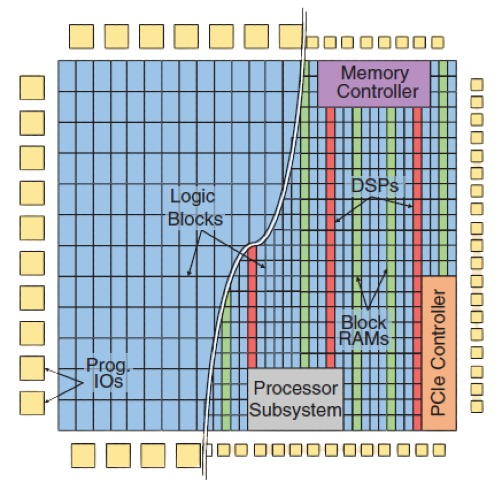
\includegraphics[scale = 0.6]{Figures/fpga_architecture.jpg}}
	\caption{FPGA Architecture Overview : Early v/s Modern\cite{boutros2021fpga}}
	\label{fig:fpga architecture}
\end{figure}

\subsection{Configurable Logic and Logic Clusters}
The smallest unit of computation in an FPGA is the Basic Logic Element (BLE), which typically comprises a K-input Lookup Table (K-LUT), a flip-flop (FF), and multiplexers to select between combinational and registered outputs. The K-LUT is a truth table stored in SRAM that can implement any K-input Boolean function. For example, a 6-LUT can encode any 6-input logic by programming 64 SRAM bits. Fig.\ref{fig:4-lut transistor} depicts the implementation of a 4-LUT at a transistor level.

\begin{figure}
	\centerline{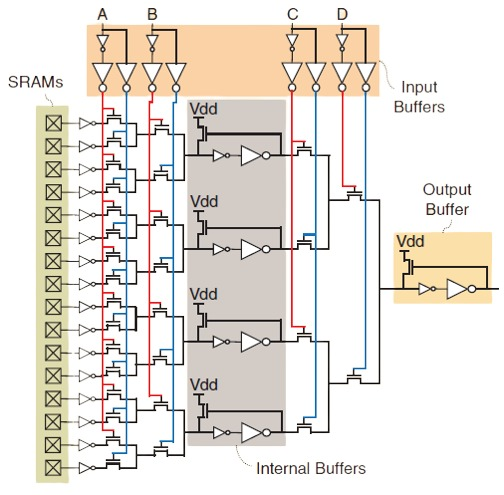
\includegraphics[scale = 0.6]{Figures/4-LUT-Transistor.jpg}}
	\caption{Transistor Implementation of a 4-LUT\cite{boutros2021fpga}}
	\label{fig:4-lut transistor}
\end{figure}

Modern BLEs implement fracturable logic to increase logic packing efficiency\cite{funda-fpga-arch-1}. A fracturable 6-LUT can operate as either a single 6-input LUT or two 5-input LUTs sharing inputs\cite{stratix2007stratix}. This flexibility reduces unused logic and enables higher performance. Intel's Adaptive Logic Modules (ALMs) and Xilinx's slice-based architectures exemplify this trend, enabling efficient use of logic resources.

BLEs are grouped into larger clusters called Logic Array Blocks (LABs) or Configurable Logic Blocks (CLBs). Each LAB may contain 8 to 32 BLEs and includes a local interconnect network for intra-block communication. This local interconnect is typically implemented using multiplexers arranged as full or partial crossbars\cite{funda-fpga-arch-2}\cite{funda-fpga-arch-3}. As the number of BLEs per LAB increases, more signal routing can be localized, reducing pressure on global routing resources and improving performance. The internal architecture of the LAB is given in Fig.\ref{fig:lab internal architecture}.

\begin{figure}
	\centerline{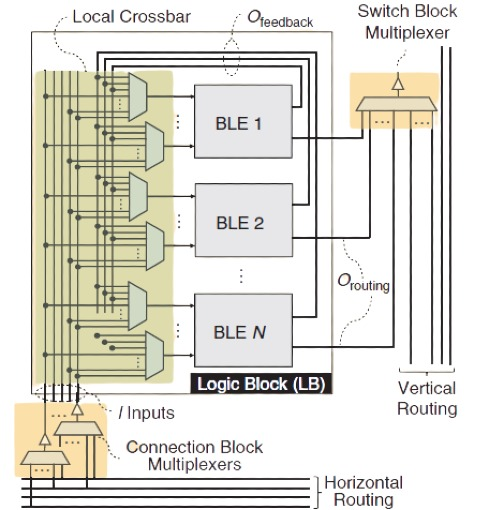
\includegraphics[scale = 0.6]{Figures/LAB-architecture.jpg}}
	\caption{LAB Internal Architecture\cite{boutros2021fpga}}
	\label{fig:lab internal architecture}
\end{figure}

The design trade-off in LAB size lies between logic utilization, routing efficiency, and critical path delay. Larger LABs reduce inter-block communication but increase complexity in placement and delay modeling.

\subsection{Programmable Routing Architecture}
The dominant routing style in modern FPGAs is the island-style architecture. In this topology, logic blocks (LABs) are arranged in a 2D grid and are surrounded by horizontal and vertical routing channels. These channels consist of wire segments of varying lengths and programmable switches.

Three main elements define the island-style routing fabric:
\begin{enumerate}
	\item \textbf{Connection Blocks:} Interface logic block I/Os to routing channels.
	\item \textbf{Switch Blocks:} Enable programmable interconnection between horizontal and vertical wires.
	\item \textbf{Wire Segments:} Allow signal propagation across the chip, often spanning 1, 4, or 16 logic blocks.
\end{enumerate}

Efficient switch block designs (e.g., Wilton pattern) and wire-length tuning reduce signal delay and area overhead\cite{funda-fpga-arch-4}. To address long-distance routing delays, modern FPGAs also employ hierarchical wiring and segment-bypassing strategies. The most popular routing style architecture, the island style routing architecture, is depicted in Fig.\ref{fig:island style routing architecture}. This style of routing is employed in the test architectures employed in the study, which we will see in the following sections.

\begin{figure}[H]
	\centerline{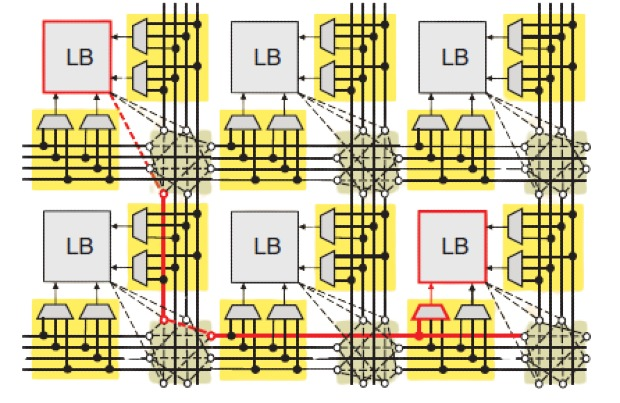
\includegraphics[scale = 0.6]{Figures/island_style_routing-removebg-preview.jpg}}
	\caption{Island Style Programmable Routing Architecture\cite{boutros2021fpga}}
	\label{fig:island style routing architecture}
\end{figure}

Programmable switches form the core of reconfigurable routing. Early designs used simple pass transistors, but these incur high resistance and delay\cite{funda-fpga-arch-5}. Buffered multiplexers are now preferred, where multiple pass transistors feed a buffer, improving speed and electrical isolation\cite{funda-fpga-arch-6}\cite{funda-fpga-arch-7}. This design limits signal injection points but significantly enhances signal integrity and performance.

\subsection{Embedded Arithmetic and Carry Chains}
Arithmetic operations such as addition and multiplication are common in FPGA workloads. Although they can be implemented with LUTs, this approach is inefficient. Instead, modern FPGAs integrate hardened arithmetic logic like carry chains directly within BLEs.

Carry chains enable fast ripple-carry and carry-skip adders. They allow the carry-out of one BLE to directly feed the carry-in of the next without passing through the general routing fabric, minimizing delay. Xilinx FPGAs use carry look-ahead logic in Versal devices, whereas Intel’s Agilex architecture implements two-bit arithmetic per logic element. These dedicated structures are optimized for speed and minimize logic usage for arithmetic-heavy workloads.

Advanced carry-chain structures like carry-skip and carry-lookahead adders are hardened to further accelerate arithmetic paths. Carry logic is commonly coupled with sum and propagate generation logic inside LUTs, and is tightly integrated into the physical layout to reduce interconnect delay. These carry networks are also exploited to accelerate custom DSP-style operators and are essential for low-precision multiply-accumulate (MAC) implementations.

These features are especially beneficial for domains requiring high arithmetic intensity, such as digital signal processing, image processing, and machine learning accelerators.

\subsection{On Chip Memory: BRAM and LUT-RAM}
To address diverse memory needs, FPGAs embed Block RAMs (BRAMs) with configurable size, depth, and access ports\cite{funda-fpga-arch-8}\cite{funda-fpga-arch-9}. A typical dual-port BRAM includes row/column decoders, sense amplifiers, and output multiplexers. Capacities range from 2Kb to 20Kb, with typical configurations supporting 1R/1W or 2R/W modes.

Peripheral logic allows BRAMs to operate in various data widths and depths (e.g., 32x64-bit or 64x32-bit)\cite{funda-fpga-arch-10}\cite{funda-fpga-arch-11}. Input/output ports are pipelined to ease timing closure, and routing interfaces are carefully optimized to reduce area and delay.

In addition to BRAMs, FPGA vendors allow LUTs to function as small distributed RAMs. By configuring LUT truth tables and adding minimal write logic, logic blocks can operate as single or dual-port LUT-RAMs (e.g., 64x10-bit). This memory is ideal for register files and coefficient storage. However, only a subset of logic blocks typically supports LUT-RAM to balance area cost\cite{funda-fpga-arch-12}.

\subsection{DSP Hard Blocks}
FPGAs embed hardened Digital Signal Processing (DSP) slices to accelerate multiply-accumulate (MAC) operations. These slices support pre-adders, multipliers, accumulators, and configurable pipelining\cite{funda-fpga-arch-13}. MACs can be cascaded to implement dot products, convolution, and matrix multiplications efficiently.

DSP slices reduce logic utilization and boost performance for compute-intensive tasks such as deep learning inference, FFTs, and image processing. 

\subsection{Programmable IO Blocks}
IOBs are specialized blocks that manage communication between the FPGA core and external devices. They support a wide range of electrical standards (e.g., LVCMOS, SSTL, LVDS) and features like:
\begin{enumerate}
	\item Programmable drive strength and slew rate
	\item On-die termination
	\item Programmable delay lines
	\item Differential signaling and serial transceivers
\end{enumerate}

Advanced IOs integrate DDR memory controllers and serial links (e.g., PCIe, Ethernet) with hardened logic. FPGA IOs are grouped into banks, each operating at configurable voltages. These features make FPGAs ideal for communication-heavy applications.

%% END OF THE SECTION - FUNDAMENTALS OF FPGA ARCHITECTURE %%

%% START OF THE SECTION - TARGET FPGA ARCHITECTURES USED IN THE STUDY %%
\section{Target FPGA Architectures Used in the Study}
This study explores and benchmarks three FPGA target architectures, each modeled using VTR (Verilog-to-Routing) XML architecture description files. These include: (1) an Intel Stratix-10-like architecture that serves as a high-performance, industry-grade baseline, and two custom arithmetic-optimized variants, namely (2) a 4-bit Single Carry Chain architecture and (3) a 4-bit Double Carry Chain architecture. Each design showcases unique internal arithmetic structures and carry chain implementations aimed at evaluating low-precision arithmetic performance, relevant to domains such as deep learning inference.

\subsection{Intel Stratix-10-like Architecture}
The Stratix-10-like architecture models a high-end commercial FPGA design. The logic fabric consists of Logic Array Blocks (LABs), each comprising 10 Adaptive Logic Modules (ALMs). Every ALM contains a 6-input Lookup Table (6-LUT) that is fracturable into two 5-LUTs, supporting rich logic packing. Each ALM exposes 8 input pins and 4 output pins, which may be optionally registered using internal flip-flops\cite{target-arch-1}. Fig.\ref{fig:stratix-10 block diagram} highlights the block diagram of Intel's Stratix-10 high level block diagram.

\begin{comment}
\begin{figure}[H]
	\centerline{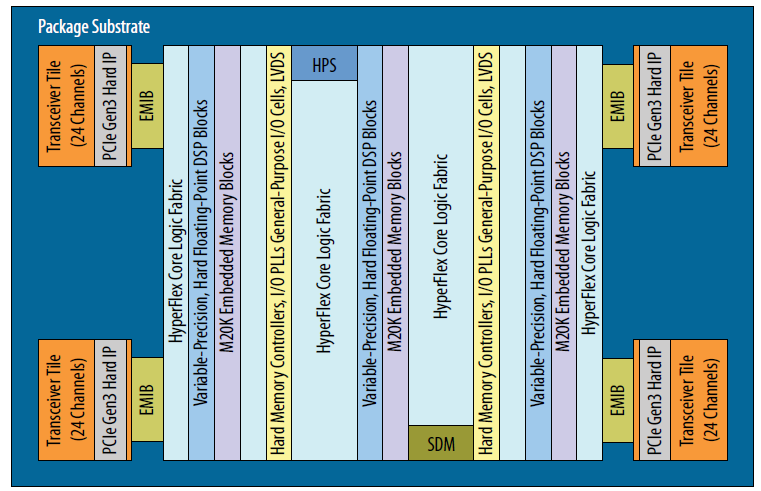
\includegraphics[scale = 0.60]{Figures/stratix_10_blockdiagram.png}}
	\caption{Intel's Stratix-10 Block Diagram}
	\label{fig:stratix-10 block diagram}
\end{figure}
\end{comment}

The key features of the Intel Stratix-10 like architecture are-
\begin{enumerate}
	\item \textbf{Arithmetic Mode Support:} Each 5-LUT can be fractured into two 4-LUTs, enabling two bits of addition per ALM in arithmetic mode. Thus, a LAB can support 20 bits of addition in a single carry chain across 10 ALMs.
	\item \textbf{Single Carry Chain:} The carry chain is linear, spanning the 10 ALMs within a LAB. The carry-out ($cout$) of one ALM feeds directly into the carry-in ($cin$) of the next, enabling fast arithmetic accumulation. 
	\item \textbf{Direct Connections:} ALM outputs feed both into neighboring LABs (left and right) and back into the LAB’s own input ports. This enhances localized reuse and dataflow.
	\item \textbf{Memory Support:} Each LAB can interface with a 20 Kb embedded RAM block, configurable in multiple true and simple dual-port modes.
	\item \textbf{DSP Integration:} A 27x27 DSP block (fracturable into 18x19 blocks) is embedded within the tile grid to support high-throughput MAC operations.
\end{enumerate}

This architecture balances general-purpose logic density with specialized arithmetic acceleration, making it suitable as a benchmark for more customized variants.

\subsection{4-bit Single Carry Chain Architecture}
This custom architecture builds on the Stratix-10 baseline but modifies the arithmetic capabilities for enhanced support of low-precision adders. It retains the same LAB structure—10 ALMs per LAB, 6-LUTs fracturable into two 5-LUTs—but introduces further fracturing into 3-LUTs\cite{target-arch-2}.

Key features of this architecture include-
\begin{enumerate}
	\item \textbf{Enhanced Arithmetic Fracturing:} In half the ALMs (ALM[0] to ALM[4]), each 5-LUT can be split into two 4-LUTs, and each 4-LUT further into two 3-LUTs. This yields 8 effective 3-LUTs per ALM, supporting 4-bit adders per ALM.
	\item \textbf{Single Carry Chain:} A single carry chain spans only the first 5 ALMs (ALM[0] to ALM[4]), providing a total of 20 bits of low-precision addition per LAB.
	\item \textbf{Optimized for Compact Arithmetic:} This configuration allows dense packing of small adders using minimal resources, reducing delay and improving energy efficiency for small-scale DSP and ML operations.
\end{enumerate}

This design evaluates how resource utilization and delay scale when packing narrow adders and embedding a shallow carry propagation chain.

\subsection{4-bit Double Carry Chain Architecture}
Expanding upon the single-chain variant, this architecture introduces a dual carry chain structure to exploit parallelism in arithmetic computation\cite{target-arch-2}.

Key features of this architecture include-
\begin{enumerate}
	\item \textbf{Double Carry Chains:} The LAB is split into two independent carry chains:
	\begin{itemize}
		\item Chain 1 spans ALM[0] to ALM[4]
		\item Chain 2 spans ALM[5] to ALM[9]
	\end{itemize}
	\item Each chain operates independently, with separate $cin$ and $cout$ ports, enabling concurrent execution of two 4-bit addition operations.
	\item \textbf{Full Arithmetic Fracturing:} Similar to the single chain, each ALM supports decomposition into eight 3-LUTs, enabling 4-bit addition within a compact area.
	\item \textbf{Routing Considerations:} The architecture includes direct interconnects between the carry-out of one LAB and the carry-in of the LAB below for each chain, supporting vertical propagation of arithmetic results.
\end{enumerate}

This configuration is ideal for evaluating parallelism vs. resource duplication trade-offs, particularly in scenarios where low-precision arithmetic operations can be concurrently dispatched, such as SIMD-style ML workloads.

\subsection{Summary of Architectural Differences}
Table.\ref{tab:fpga architectural differences between test architectures} summarizes the architectural differences between the Intel Stratix-10-like, 4-bit single carry chain and 4-bit double carry chain architectures.
% TABLE TO PRESENT THE ARCHITECTURAL DIFFERENCES
\begin{comment}
\begin{table}[ht]
	\centering
	\fontsize{10}{12}\selectfont
	\caption{FPGA Architectural Differences between Test Architectures}
	\scalebox{0.65}{
		\begin{tabular}{|c|c|c|c|}
			\hline
			\textbf{Feature} & \textbf{Stratix-10-like} & \textbf{4-Bit Single Chain} & \textbf{4-Bit Double Chain}\\
			\hline
			%\hline
			ALMs per LAB & 10 & 10 & 10 \\
			\hline
			Fracturable LUT Structure & 6-LUT to 5-LUT to 4-LUT & 6-5-4-3 LUT (half ALMs) & 6-5-4-3 LUT (all ALMs) \\
			\hline
			Carry Chains & 1 full LAB wide & 1 in ALM[0] to ALM[4] & 2 (ALM[0-4] and ALM[5-9]) \\
			\hline
			Arithmetic Parallelism & Sequentual & Narrow Serial (5 ALMs) & Dual Parallel Chains \\
			\hline
			Target Use-Case & General Logic and DSP & Low Precision MACs & Parallelized Arithmetic \\
			\hline
	\end{tabular}}
	
	%\label{tab:fpga architectural differences between test architectures}
\end{table}
\end{comment}

\begin{table}[htb]
	\fontsize{10}{12}\selectfont
	\caption{FPGA Architectural Differences between Test Architectures}
	\label{tab:fpga architectural differences between test architectures}
	\begin{tabular}{|p{3cm}|c|c|c|}
		%\hline
		%\multicolumn{4}{|c|}{Country List} \\
		\hline
		\textbf{Feature}& \textbf {Stratix-10-Like} & \textbf {4-Bit Single Chain} & \textbf{4-Bit Double Chain}\\
		\hline
		ALMs per LAB & 10 & 10 & 10\\\hline
		Fracturable LUT Structure & 6-LUT to 5-LUT to 4-LUT & 6-5-4-3 LUT (half ALMs) & 6-5-4-3 LUT (all ALMs) \\\hline
		Carry Chains & 1 full LAB wide & 1 in ALM[0] to ALM[4] & 2 (ALM[0-4] and ALM[5-9]) \\\hline
		Arithmetic Parallelism & Sequentual & Narrow Serial (5 ALMs) & Dual Parallel Chains \\\hline
		Target Use-Case & General Logic and DSP & Low Precision MACs & Parallelized Arithmetic \\\hline
	\end{tabular}
\end{table}

These architectures provide a valuable testbed for understanding how architectural customization affects logic packing, delay, and arithmetic throughput in FPGA-based computation.

%% END OF THE SECTION - TARGET FPGA ARCHITECTURES USED IN THE STUDY %%

%% START OF THE SECTION - HDL BENCHMARKS EMPLOYED IN THE STUDY %%
\section{HDL Benchmarks Employed in the Study}
This study utilizes a series of parameterized Verilog benchmarks to evaluate the synthesis, placement, routing, and delay characteristics of different FPGA architectures under arithmetic and signal processing workloads. These benchmarks are representative of typical low-level compute patterns found in many machine learning and digital signal processing (DSP) applications. Each benchmark is crafted to stress particular architectural resources such as carry chains, routing networks, and DSP blocks. The categories are described below.

\subsection{2-Level Adder Trees}
The 2-level adder tree benchmark represents a fundamental building block for arithmetic reductions and accumulation operations. It takes eight parallel inputs, grouped in binary pairs, and recursively sums them in a two-level hierarchy using combinational adders. The structure implements three layers:
\begin{enumerate}
	\item \textbf{Level 3:} Performs four pairwise additions of the eight inputs.
	\item \textbf{Level 2:} Aggregates the four intermediate results into two partial sums.
	\item \textbf{Level 1:} Produces the final result from the two intermediate sums. 	
\end{enumerate}

Each addition stage is implemented using a generic adder-tree-branch module with a configurable EXTRA-BITS parameter to accommodate bit growth through each level of the hierarchy. The bit-width of inputs is configurable, enabling stress-testing across low- to medium-precision operand sizes.

This design serves as an effective benchmark for:
\begin{enumerate}
	\item \textbf{Carry chain utilization:} As each addition requires ripple or look-ahead carry logic.
	\item \textbf{Critical path analysis:} Timing accumulates from multiple levels of combinational logic.
	\item \textbf{Area-delay tradeoffs:} Bit growth and tree depth impact routing congestion and synthesis area.
\end{enumerate}

The register stages at the input ensure timing closure under a pipelined regime, and the configuration can be toggled to emulate either 2-level or 3-level adder behavior, providing flexibility in benchmarking deeper vs. shallower arithmetic pipelines.

\subsection{3-Level Adder Trees}
The 3-level adder tree benchmark extends the arithmetic hierarchy of the 2-level design, implementing a complete three-stage binary reduction to compute the sum of eight input operands. Each operand is of configurable bit-width, allowing this benchmark to target multiple datapath sizes typically encountered in hardware accelerators, such as in digital signal processing (DSP) or MAC (multiply-accumulate) structures in ML workloads.

The benchmark operates in the following sequence:
\begin{enumerate}
	\item \textbf{Level 3:} Computes four pairwise sums from the eight input signals.
	\item \textbf{Level 2:} Takes the four L3 results and reduces them to two partial sums.
	\item \textbf{Level 1:} Produces the final output by summing the two L2 outputs.
\end{enumerate}

Each stage employs a parameterized adder-tree-branch that accounts for bit growth due to binary addition. This is controlled via the EXTRA-BITS parameter, which increases by one bit per level to prevent overflow and maintain accuracy.

Notable features of the 3-level adder trees include:
\begin{enumerate}
	\item \textbf{Fully Combinational Addition Path:} Unlike pipelined designs, this benchmark computes the final output purely through combinational logic from the input stage to the output in a single cycle, stressing the critical path delay.
	\item \textbf{Stress on Carry Chains:} The deeper hierarchy increases the load on carry propagation networks, allowing accurate benchmarking of architectures with varying carry chain optimizations (e.g., single vs. double chain).
	\item \textbf{Bit-Width Scalability:} The design is generic across operand sizes (e.g., 4-bit, 8-bit, 16-bit) and models how delay and logic utilization scale with increasing precision.
\end{enumerate}

The 3-level tree structure is representative of workloads requiring high fan-in reductions, such as in deep learning accumulators, dot product units, and reduction phases of sum-pooling layers. It also provides insight into how FPGA routing and LUT utilization scale with deeper arithmetic pipelines, and how carry propagation affects synthesis timing.

\subsection{Unpipelined FIR Filter with Hardblock Multipliers}
This benchmark models a classic Finite Impulse Response (FIR) filter implemented in an unpipelined configuration using dedicated DSP hardblocks for multiplication. It emulates a 10-tap symmetric FIR filter, which leverages the property of coefficient symmetry to reduce computational redundancy by only requiring five unique coefficients. The architecture processes a sliding window of ten input samples, pairing symmetric inputs and summing them in a series of five initial additions. These pairwise sums are subsequently multiplied by the respective filter coefficients using multiplier units, assumed to map directly to FPGA DSP slices (e.g., 18×18 or 27×18 multipliers).

The multiplication outputs are then passed through a multi-level adder tree, where they are combined using a series of registered addition modules to produce the final output. Although input and output registers are present for signal stability and timing, the computation pipeline itself remains unpipelined. As such, the entire multiply-accumulate (MAC) computation occurs in a combinational path with sequential output capture, stressing the design's critical path and highlighting the FPGA architecture's ability to meet timing without deeper pipelining. Control flow is managed using a valid-signal propagation pipeline to ensure data consistency across the input and output stages.

This benchmark is essential for evaluating how an FPGA architecture handles computationally intensive DSP workloads without the benefits of pipelining. It is particularly useful for analyzing critical path delays, synthesis area, logic and DSP block utilization, and the efficiency of routing under MAC-dominated loads. Moreover, the benchmark provides a reference point for comparing with pipelined implementations in terms of latency, throughput, and resource efficiency, especially in applications where minimizing dynamic power or leveraging dedicated multipliers is a key design goal.

\subsection{Pipelined FIR Filter with Hardblock Multipliers}
The pipelined FIR filter benchmark builds upon the foundational structure of its unpipelined counterpart but introduces staged computation through register insertion, enabling improved throughput and deeper timing closure. This design also implements a symmetric 10-tap FIR filter with five unique coefficients and exploits coefficient symmetry to minimize the number of multiplications required. Input samples are processed through a shift register pipeline, from which symmetric pairs are summed and then multiplied with corresponding coefficients using dedicated hardware multipliers that align with DSP blocks typically available in commercial FPGA fabrics.

What distinguishes this version from the unpipelined design is the strategic placement of registers between every major computational stage—after the symmetric additions, after each multiplication, and throughout the reduction adder tree. These pipelining registers help shorten critical paths and allow the design to run at higher clock frequencies, making it more suitable for high-throughput applications such as real-time signal processing or embedded ML inference. Each computation level performs only a small segment of the total work per clock cycle, resulting in reduced combinational delay and improved timing characteristics.

The control pipeline tracks data validity using a dedicated valid signal shift register, which aligns output generation with the pipeline depth. This structured staging increases latency slightly due to the additional cycles required for data propagation through each stage, but it greatly enhances throughput as new inputs can be accepted every clock cycle. This benchmark is ideal for evaluating how well an FPGA architecture supports pipelined arithmetic workloads, especially in terms of logic utilization, DSP block efficiency, and register overhead. Moreover, it demonstrates how architectural pipelining can be leveraged to scale MAC-intensive operations while maintaining high operating frequencies.

\subsection{Unpipelined FIR Filter with Carry Chains}
This variant of the unpipelined FIR filter is structurally identical to its hardblock-based counterpart but replaces dedicated multipliers with synthesized Wallace tree multipliers constructed entirely from single-bit adders. By decomposing the multiplication operation into a series of partial product generations and reductions, this design shifts the computational burden from DSP blocks to the FPGA's general-purpose logic fabric—specifically the carry chains. The benchmark still implements a symmetric 10-tap FIR filter using five unique coefficients, with input samples processed through a sliding window and summed in symmetric pairs. However, each multiplication is replaced by an 18-bit Wallace tree multiplier composed of carry-optimized addition layers.

This architectural substitution significantly alters the behavior of the design with respect to synthesis and timing. Instead of mapping to dedicated DSP slices, the design now stresses the carry propagation network and LUT fabric, especially in architectures optimized for low-precision arithmetic via enhanced carry chain logic. Without pipelining, all levels of the multiply-accumulate (MAC) computation execute within a single clock cycle. As a result, the critical path is dominated by the depth of the Wallace tree multiplier and subsequent adder stages, providing a valuable stress test for logic delay and routing complexity in FPGA fabrics.

This benchmark is particularly useful for evaluating how well an FPGA architecture supports synthesized arithmetic under carry-intensive workloads. It reveals the relative efficiency of different carry chain implementations—such as single vs. double carry chains—and the extent to which these optimizations impact timing closure and logic density. Moreover, by replicating a DSP workload using general logic resources, this test exposes trade-offs between logic usage and DSP conservation, especially in scenarios where hardblocks are limited or reserved for higher-precision operations.

\subsection{Pipelined FIR Filter on Carry Chains}
This FIR benchmark extends the carry chain-based multiplier implementation by introducing a fully pipelined computation structure, enabling higher clock frequencies and improved throughput. As in the unpipelined version, the core multiplication operations are synthesized using Wallace tree multipliers built from single-bit adders, rather than utilizing dedicated DSP hardblocks. These multipliers rely on layers of carry chain-accelerated adders to construct 18-bit multiplication results through partial product accumulation and reduction. The FIR filter retains a 10-tap symmetric structure with five unique coefficients, and input samples are processed through a series of shift registers that maintain a sliding window of data.

Each stage of the computation—from the symmetric additions and Wallace tree multipliers to the reduction adder tree—is separated by clocked register stages, creating a deeply pipelined data path. This staged computation reduces the depth of combinational logic per cycle and enables the design to meet tighter timing constraints on FPGA fabrics. The use of carry chain-based Wallace multipliers allows the design to test the efficiency of FPGA logic structures in scenarios where DSP blocks are not available or are reserved for other purposes. The output valid signal is aligned with the data path using a pipelined control register, ensuring synchronized streaming of results.

This benchmark is highly illustrative of how FPGAs can be leveraged to perform DSP-style operations purely using general-purpose logic and carry chains. It stresses not only the FPGA's carry propagation infrastructure but also its ability to maintain high throughput under deep pipelining. The design is particularly relevant for evaluating low-precision arithmetic acceleration strategies, where resource efficiency and carry chain utilization directly impact performance and power efficiency.

The pipelined FIR filter benchmark builds upon the foundational structure of its unpipelined counterpart but introduces staged computation through register insertion, enabling improved throughput and deeper timing closure. This design also implements a symmetric 10-tap FIR filter with five unique coefficients and exploits coefficient symmetry to minimize the number of multiplications required. Input samples are processed through a shift register pipeline, from which symmetric pairs are summed and then multiplied with corresponding coefficients using dedicated hardware multipliers that align with DSP blocks typically available in commercial FPGA fabrics.

What distinguishes this version from the unpipelined design is the strategic placement of registers between every major computational stage—after the symmetric additions, after each multiplication, and throughout the reduction adder tree. These pipelining registers help shorten critical paths and allow the design to run at higher clock frequencies, making it more suitable for high-throughput applications such as real-time signal processing or embedded ML inference. Each computation level performs only a small segment of the total work per clock cycle, resulting in reduced combinational delay and improved timing characteristics.

The control pipeline tracks data validity using a dedicated valid signal shift register, which aligns output generation with the pipeline depth. This structured staging increases latency slightly due to the additional cycles required for data propagation through each stage, but it greatly enhances throughput as new inputs can be accepted every clock cycle. This benchmark is ideal for evaluating how well an FPGA architecture supports pipelined arithmetic workloads, especially in terms of logic utilization, DSP block efficiency, and register overhead. Moreover, it demonstrates how architectural pipelining can be leveraged to scale MAC-intensive operations while maintaining high operating frequencies.

%% END OF THE SECTION - HDL BENCHMARKS EMPLOYED IN THE STUDY %%

%% START OF THE SECTION - ARCHITECTURE-BENCHMARK EVALUATIION METRICS %%
\section{Architecture-Benchmark Evaluation Metrics}
To evaluate the effectiveness of each FPGA architecture under study, a set of quantitative metrics were employed to characterize the performance and resource efficiency of the HDL benchmarks mapped onto them. The primary metrics considered are operational frequency, area (in Minimum Width Transistor Area or MWTA units), and critical path delay. These parameters provide a holistic view of architectural efficiency in supporting arithmetic and signal-processing-dominated hardware designs.

Operational Frequency denotes the maximum clock speed at which the synthesized design can function reliably. It is influenced by logic depth, routing congestion, and architectural support for pipelining and carry propagation. A higher operational frequency typically reflects better timing closure, which is crucial for real-time ML inference and high-throughput data processing.

Area in MWTA units represents the physical resource cost of implementing the benchmark design on the FPGA fabric\cite{arch-benchmark-metrics-1}. It quantifies the required logic, routing, and hard block utilization in terms of minimum-width transistor area equivalents, providing a normalized view of silicon efficiency. Area optimization is especially relevant in ML accelerators where packing more compute units per chip can dramatically improve inference throughput.

Critical Path Delay, measured in nanoseconds, refers to the longest propagation delay between input and output in the combinational logic path\cite{arch-benchmark-metrics-2}. It directly impacts the achievable clock frequency and therefore the latency of computations. Designs with deep carry chains, long adder trees, or complex multiplier logic tend to have higher critical path delays. Reducing this delay is crucial for supporting low-latency ML tasks, such as real-time vision or audio processing.

Collectively, these metrics allow for meaningful comparisons between FPGA architectures with varying logic organization, carry chain capabilities, and hard block integration. In the context of machine learning hardware, where latency, throughput, and energy efficiency are paramount, these metrics help identify architectural features that offer superior trade-offs for different classes of ML workloads.

%% END OF THE SECTION - ARCHITECTURE-BENCHMARK EVALUATIION METRICS %%

%% START OF THE SECTION - VTR TOOLCHAIN %%
\section{VTR Toolchain}
The Verilog-to-Routing (VTR) toolchain is an open-source CAD framework developed to explore FPGA architecture, CAD algorithms, and mapping strategies through end-to-end synthesis and implementation. Its modular and customizable structure makes it a powerful platform for academic and experimental research into FPGA logic structures, placement and routing techniques, and architecture-aware optimizations\cite{vtr-toolchain-1}\cite{target-arch-2}.

The motivation behind VTR is to bridge the gap between Verilog-based digital design and physical FPGA layout analysis. It enables rapid prototyping and benchmarking of custom FPGA architectures without relying on proprietary tools, allowing researchers to test architectural modifications such as specialized carry chains, fracturable LUTs, or heterogeneous hard block integration.

The VTR CAD flow, as shown in Fig.\ref{fig:vtr cad flow} begins with Verilog input and proceeds through synthesis, logic optimization, technology mapping, packing, placement, routing, and final analysis. This sequence emulates a full CAD flow while offering hooks for architectural experimentation at each stage.

\begin{figure}
	\centerline{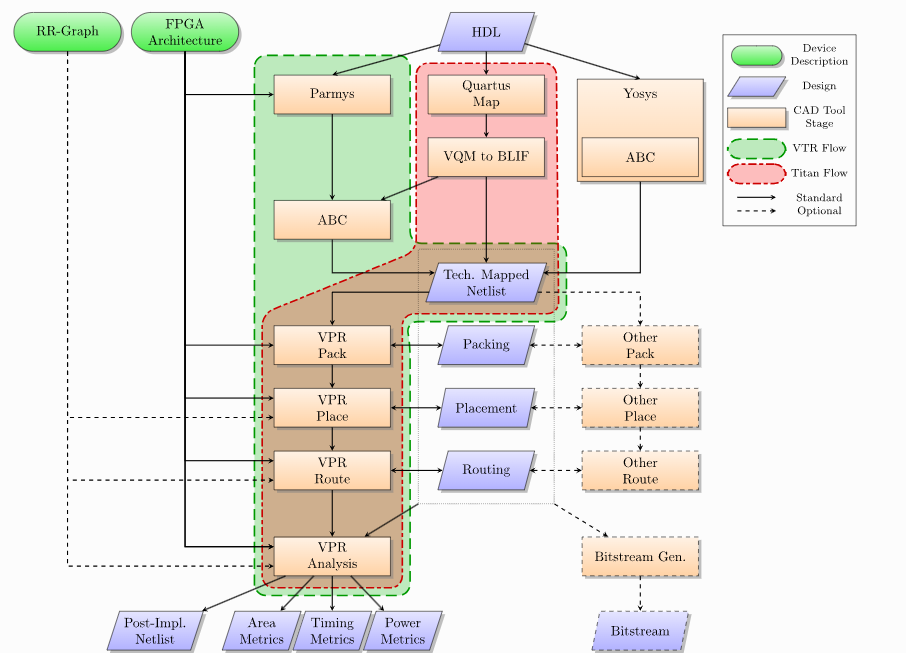
\includegraphics[scale = 0.8125]{Figures/vtr_cad_flow.png}}
	\caption{VTR CAD Flow\cite{vtr-toolchain-1}}
	\label{fig:vtr cad flow}
\end{figure}

The flow begins with Yosys, an open-source Verilog synthesis suite\cite{vtr-toolchain-2}. Yosys parses the Verilog HDL, performs initial optimizations, and generates a structural netlist in BLIF (Berkeley Logic Interchange Format), a textual format that represents gate-level designs. BLIF is widely used as a standard intermediate format in logic synthesis and academic CAD tools.

The generated BLIF netlist is then passed to ABC, a logic optimization and technology mapping tool developed at UC Berkeley\cite{vtr-toolchain-3}. ABC performs logic restructuring and maps logic functions onto basic gate primitives compatible with FPGA LUTs\cite{vtr-toolchain-4}. It also reduces logic depth and performs retiming optimizations where applicable. The output of ABC is a further optimized BLIF file used by VTR's core tools.

Next, the VPR (Versatile Place and Route) engine takes over. VPR performs three major tasks:
\begin{enumerate}
	\item \textbf{Packing:} Groups logic elements (e.g., LUTs, FFs) into logic clusters (CLBs or LABs) based on FPGA architecture constraints.
	\item \textbf{Placement:} Assigns packed logic clusters to specific physical locations in the FPGA grid.
	\item \textbf{Routing:} Connects placed logic blocks using the programmable interconnect and switch boxes, while adhering to the routing architecture defined in the FPGA model.
\end{enumerate}

VPR concludes with analysis, reporting timing, area (in MWTA), and power estimates. These results form the basis for comparative benchmarking of various architecture configurations\cite{vtr-toolchain-5}.

One of VTR’s most powerful features is its architecture description framework. Custom FPGA architectures are described using XML files that specify logic block structures, interconnect topologies, routing switch types, I/O standards, timing models, and cluster configurations. These XML descriptions are parsed and interpreted by VPR, enabling researchers to design and evaluate unconventional architectures—such as carry-chain-enhanced FPGAs, multi-CLB tiles, or DSP-rich fabrics—without modifying the underlying toolchain source code.

Overall, the VTR toolchain provides a complete, transparent, and configurable flow that is essential for academic research and architectural benchmarking. Its integration of synthesis, logic mapping, placement, and routing, combined with custom architecture support, makes it an indispensable framework for the exploration and evaluation of FPGA designs tailored for emerging compute workloads like machine learning.

%% END OF THE SECTION - VTR TOOLCHAIN %%

%% START OF THE SECTION - FUNDAMENTALS OF PRINCIPAL COMPONENT ANALYSIS
\section{Principal Component Analysis (PCA)}
\subsection{Introduction and Evaluation Metrics}
Principal Component Analysis (PCA) is a statistical method used to transform a set of correlated variables into a new set of uncorrelated variables known as principal components. These components are linear combinations of the original variables, arranged in order of decreasing variance. The primary goal of PCA is to identify the most significant patterns within the data while reducing its dimensionality, which is particularly useful in scenarios where data interpretation, visualization, and computational efficiency are essential. The essence of PCA lies in projecting high-dimensional data onto a new coordinate system where the dimensions are ranked based on their contribution to the dataset's overall variance\cite{pca-1}\cite{pca-2}.

PCA is an unsupervised learning technique widely used in machine learning, computer vision, and scientific computing. It is especially valuable in dealing with datasets where multicollinearity exists, meaning that features are highly correlated. By identifying a new set of orthogonal basis vectors, PCA effectively removes redundancy and ensures that each principal component captures distinct, non-overlapping information about the dataset\cite{pca-3}. This is particularly beneficial in applications such as image compression, where PCA enables a significant reduction in the number of pixels required to reconstruct an image while preserving its essential structure, and in finance, where it helps identify latent factors influencing asset prices.

Consider a multi-feature dataset comprising M records and N features. Then, the PCA algorithm begins by standardizing the dataset to ensure that each feature contributes equally to the analysis. This involves subtracting the mean of each feature and dividing by its standard deviation, thereby transforming the data into a zero-mean, unit-variance form. Next, the covariance matrix, an NxN symmetric matrix capturing the pairwise relationships between features, is computed. This matrix provides insight into how different features vary with respect to one another. Following this, the eigenvalues and eigenvectors of the covariance matrix are determined through eigenvalue decomposition or Singular Value Decomposition (SVD). The eigenvectors represent the principal components—orthogonal directions in feature space along which data exhibits maximum variance—while the corresponding eigenvalues indicate the amount of variance captured by each component. The eigenvalues are then sorted in descending order, and the top k eigenvectors (corresponding to the largest eigenvalues) are selected to form a reduced k-dimensional subspace. Finally, the original dataset is projected onto these principal components, yielding a transformed representation where the most significant variance is retained while reducing the overall dimensionality.

The algorithm for PCA is given below-
\begin{enumerate}
	\item \textbf{Input:} Input dataset D with M rows and N features
	\item Center the dataset : For every feature, subtract the mean of the feature from each point to center the dataset about the mean
	\( x_{i} \longleftarrow x_{i} - \frac{1}{N}\sum x_{k} \)
	\item Compute the covariance matrix of the scaled down dataset
	\( C = X^{T}X \), where \( X^{T} \) is the transpose of the input dataset and Xis the input dataset
	\item Perform Singular Value Decomposition (SVD) on the covariance matrix C to procure the eigenvalues and eigenvectors of the covariance matrix \( C = VD^{2}V^{T} \), where V is the matrix whose columns are the eigenvectors of the covariance matrix and D is the diagonal matrix whose elements are the square of the eigenvalues
	\item Multiplying X and V would result in the principal components, and the eigenvectors of the top k eigenvalues are selected as the principal components
	\item \textbf{Output: } Required Principal Components from the Input dataset
\end{enumerate}

Once the eigenvalues and their corresponding eigenvectors have been computed, the next crucial step in PCA is selecting the appropriate number of principal components, k, that will effectively reduce the dimensionality while preserving most of the data's variance. There are two widely used methods for determining k: the variance contribution ratio and the cumulative variance contribution ratio\cite{pca-4}.

The variance contribution ratio (VCR) is a measure of how much variance each principal component explains relative to the total variance in the data. Given that PCA aims to retain the most significant patterns in the dataset, components with higher variance contributions are more valuable. The variance contribution ratio for the \( i^{th} \) principal component is given by:

\begin{equation}
	\label{eq:equation_1}
	P_i = \frac{\lambda_i}{\sum_{k = 1}^N\lambda_k}
\end{equation}

where \( i \) is the eigenvalue associated with the \( i^{th} \) principal component, and \( \sum_{k = 1}^N\lambda_k \) is the sum of all eigenvalues, which is directly proportional to the total variance of the dataset. By sorting the eigenvalues in descending order, the first few principal components will have the highest variance contribution ratios. Typically, a threshold is set, and only the components with a variance contribution above this threshold are retained. For instance, if the first three components have variance contributions of 40\%, 30\%, and 15\%, a common heuristic might be to select the first two or three components since they contribute the most to the total variance.

Instead of analyzing individual variance contributions, the cumulative variance contribution ratio (CVCR) provides a more holistic criterion for choosing k. It sums the variance contributions of the top k principal components to ensure that a sufficient proportion of the total variance is preserved. The cumulative variance contribution ratio for the top k components is given by:

\begin{equation}
	\label{eq:equation_3}
	CP_i = \frac{\sum_{k = 1}^i \lambda_k}{\sum_{k = 1}^N \lambda_k}
\end{equation}

The goal is to select k such that $CVCR_{k}$ exceeds a predefined threshold, typically 95\% or 99\%. This ensures that the selected principal components retain most of the dataset's variance while reducing dimensionality.

For example, suppose the cumulative variance contribution for the first four principal components is 85\%, 92\%, 97\%, and 99\%. If an application requires at least 95\% variance retention, selecting the first three components would be sufficient.

In real-world scenarios, a scree plot (a plot of eigenvalues versus component index) is often used to visualize variance contributions. The "elbow point" of this plot, where eigenvalues begin to level off, serves as an intuitive indicator of an appropriate k. Alternatively, domain-specific constraints, computational efficiency considerations, and the trade-off between information preservation and dimensionality reduction influence the final choice of k.

\subsection{Case Study on Principal Component Analysis}
As an example, consider the wine dataset from the University of California-Irvine’s ML repository\cite{pca-5}. The Wine Recognition dataset from the UCI Machine Learning Repository is a classic classification dataset used to distinguish between three varieties of wine grown in the same region of Italy. Based on the results of chemical analysis, each sample represents a wine derived from one of the three cultivars. The dataset aims to evaluate how well different physicochemical characteristics can be used to identify the grape variety. The dataset comprises of the below feature set, as shown in Table.\ref{tab:summary of original features}.

\begin{table}[h]
	\centering
	\fontsize{10}{12}\selectfont
	\caption{Summary-Original Features}
	\label{summary of original features}
	\begin{tabular}{|p{3cm}|c|c|l|}
		\hline
		\textbf{S.No} & \textbf{Feature Index} & \textbf{Feature}\\
		\hline
		%\hline
		1 & F1 & Alcohol\\
		\hline
		2 & F2 & Malic Acid\\
		\hline
		3 & F3 & Ash\\
		\hline
		4 & F4 & Alcalinity of Ash\\
		\hline
		5 & F5 & Magnesium\\
		\hline
		6 & F6 & Total Phenols\\
		\hline
		7 & F7 & Flavanoids\\
		\hline
		8 & F8 & Non flavanoid phenols\\
		\hline
		9 & F9 & Proanthocyanins\\
		\hline
		10 & F10 & Color Intensity\\
		\hline
		11 & F11 & Hue\\
		\hline
		12 & F12 & OD280 / OD315 for diluted wines\\
		\hline
		13 & F13 & Proline\\
		\hline
	\end{tabular}
	
	\label{tab:summary of original features}
\end{table}

Then, the covariance matrix of the dataset, providing an overview on the inter dependencies between the different features in the dataset, is shown in the Figure \ref{the covariance matrix}
% Covariance Matrix Image
\begin{figure}[H]
	\centerline{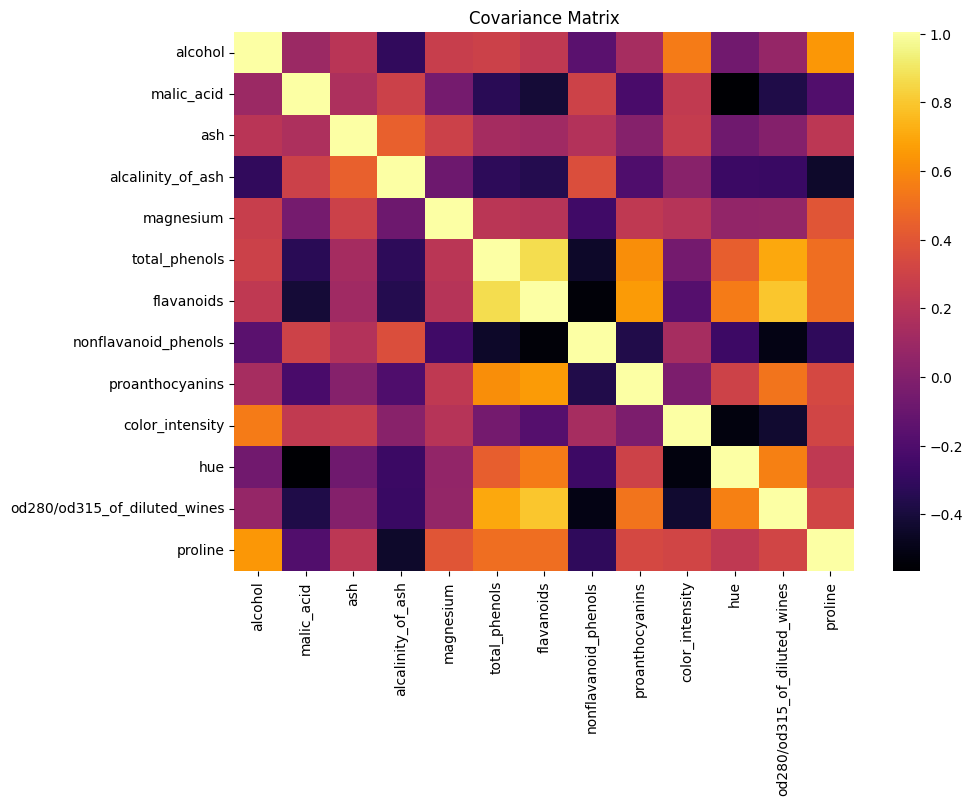
\includegraphics[scale = 0.8125]{Figures/covariance_matrix.png}}
	\caption{Covariance Matrix}
	\label{the covariance matrix}
\end{figure}

Further, the covariance matrix is decomposed into its eigenvalues and eigenvectors using Singular Value Decomposition, and the EVCR and CVCR across all the eigenvalues are calculated after arranging them in the descending order of their magnitude. Analysis of the variance contribution and cumulative variance contribution plots yield that the first 6 principal components would suffice and explain 80\% of the variance of the dataset.

The eigenvalues of the covariance matrix are computed and displayed in Table \ref{tab:eigenvalues of covariance matrix}. The eigenvectors corresponding to the top \textit{k} eigenvalues are obtained. The choice of \textit{k} will depend on the plot of explained variance ratio v/s the number of principal components chosen as shown in Figure \ref{pca ratio plot}

\begin{table}[h]
	\centering
	\fontsize{10}{12}\selectfont
	\caption{Eigenvalues of Covariance Matrix}
	\label{tab:eigenvalues of covariance matrix}
	\begin{tabular}{|p{3cm}|c|}
		\hline
		\textbf{PC\textsubscript{i}} & \textbf{Eigenvalue} \\
		\hline
		%\hline
		PC1 & 4.706\\
		\hline
		PC2 & 2.497\\
		\hline
		PC3 & 1.446\\
		\hline
		PC4 & 0.919\\
		\hline
		PC5 & 0.853\\
		\hline
		PC6 & 0.642\\
		\hline
		PC7 & 0.551\\
		\hline
		PC8 & 0.348\\
		\hline
		PC9 & 0.289\\
		\hline
		PC10 & 0.251\\
		\hline
		PC11 & 0.226\\
		\hline
		PC12 & 0.169\\
		\hline
		PC13 & 0.103\\
		\hline
	\end{tabular}
	
	\label{table:3}
\end{table}

The variance contribution ratio and the cumulative variance contribution ratio are calculated and displayed in Table \ref{variance contribution ratio of the principal components}. The line in Figure \ref{pca ratio plot} represents the principal component variance contribution ratio v/s the number of principal components chosen while the bars highlight the cumulative variance contribution ratio v/s the number of components chosen. It is seen that both the plots tend to saturate at higher principal components. Thus, it can be concluded that the first few principal components explain the majority of the data-set while the contribution of variance explained by the higher principal components is very less.

\begin{table}[h]
	\centering
	\fontsize{10}{12}\selectfont
	\caption{Variance and cumulative ratios}
	\label{table:4}
	\label{variance contribution ratio of the principal components}
	\begin{tabular}{|p{3cm}|c|c|}
		\hline
		\textbf{PC\textsubscript{i}} & \textbf{P\textsubscript{i}} & \textbf{CP\textsubscript{i}} \\
		\hline
		%\hline
		PC1 & 0.362 & 0.362\\
		\hline
		PC2 & 0.192 & 0.554\\
		\hline
		PC3 & 0.111 & 0.665\\
		\hline
		PC4 & 0.071 & 0.736\\
		\hline
		PC5 & 0.066 & 0.802\\
		\hline
		PC6 & 0.049 & 0.851\\
		\hline
		PC7 & 0.042 & 0.893\\
		\hline
		PC8 & 0.027 & 0.920\\
		\hline
		PC9 & 0.022 & 0.942\\
		\hline
		PC10 & 0.020 & 0.962\\
		\hline
		PC11 & 0.017 & 0.979\\
		\hline
		PC12 & 0.013 & 0.992\\
		\hline
		PC13 & 0.008 & 1\\
		\hline
	\end{tabular}
\end{table}

% INSERT VARIANCE CONTRIBUTION PLOTS FIGURE HERE
\begin{figure}[H]
	\centerline{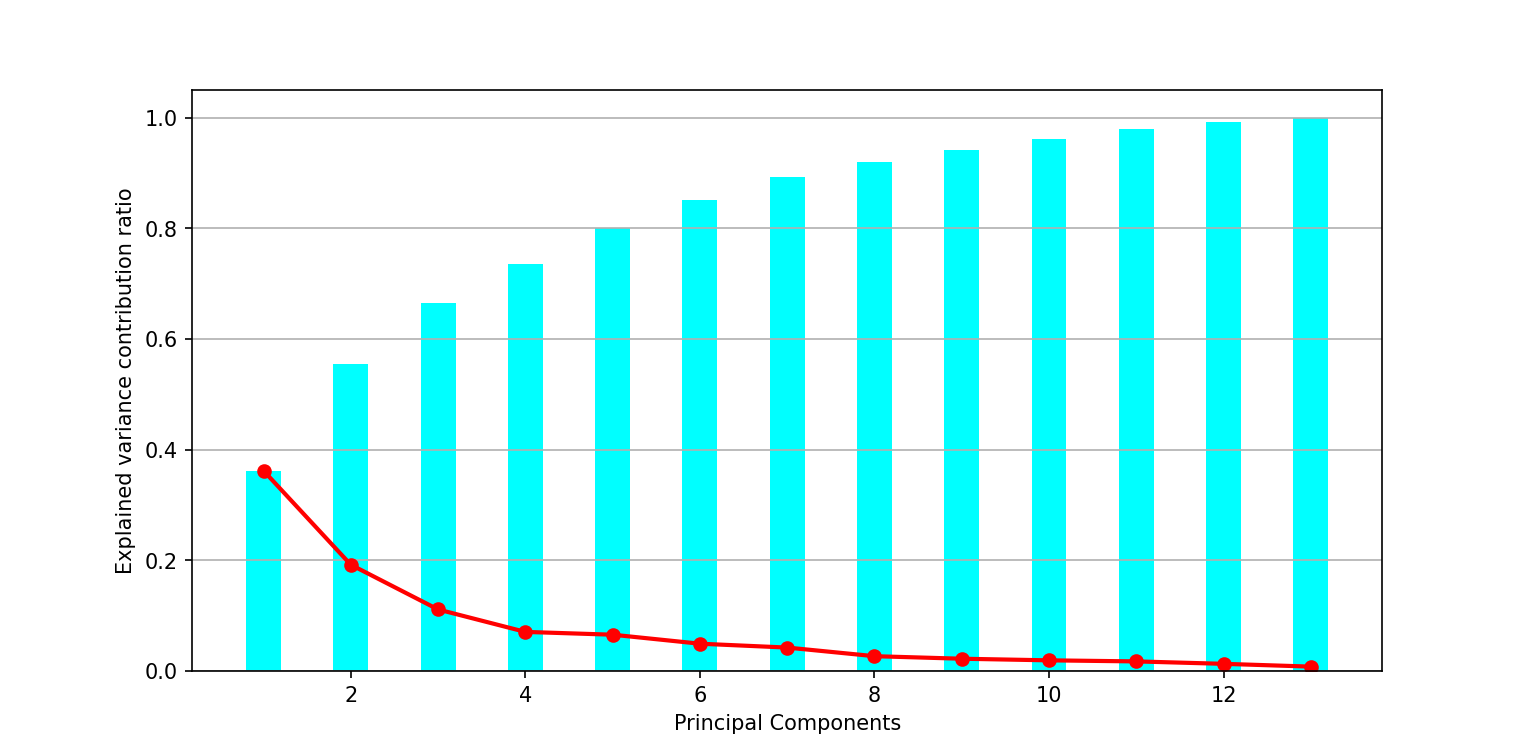
\includegraphics[scale = 0.75]{Figures/variance graph 2.png}}
	\caption{PCA Ratio Plot}
	\label{pca ratio plot}
\end{figure}

As 80\% of the variance can be captured from the first 5 principal components, the processed dataset with the first 5 principal components can be displayed in Table \ref{table:3}.

\begin{table}[h]
	\centering
	\caption{PCA Processed Table : First 5 records}
	\begin{tabular}{|p{3cm}|c|c|c|c|c|}
		\hline
		\fontsize{10}{12}\selectfont
		\textbf{S.No} & \textbf{PC1} & \textbf{PC2} & \textbf{PC3} & \textbf{PC4} & \textbf{PC5}\\
		\hline
		%\hline
		1 & 3.316751 & -1.443463 & -0.165739 & -0.215631 & 0.693043\\
		\hline
		2 & 2.209465 & 0.333393 & -2.026457 & -0.291358 & -0.257665\\
		\hline
		3 & 2.516740 & -1.031151 & 0.982819 & 0.724902 & -0.251033\\
		\hline
		4 & 3.757066 & -2.756372 & -0.176192 & 0.567983 & -0.311842\\
		\hline
		5 & 1.008908 & -0.869831 & 2.026688 & -0.409766 & 0.298458\\
		\hline
	\end{tabular}
	
	\label{table:5}
\end{table}


%% END OF THE SECTION - FUNDAMENTALS OF PRINCIPAL COMPONENT ANALYSIS %%


\begin{comment}
This chapter should discuss about the prerequisite learnings before the execution of the project. Organise and elaborate the theory and necessary fundamentals required for the execution of the project. You can use \verb|\subsections| and \verb|subsubsections| in this chapter.
\section{Contents of this chapter}
If a specific programming language is required for the project, a section can be allotted in this chapter to discuss it. 
\section{Contents of this chapter}
Tools used could be another possible section to discuss about the software tools used in the work. 
\section{Contents of this chapter}
The details in this chapter can be added in consultation with the project guide. For an internship based projects, subsections can be modified accordingly. 
\end{comment}

%% START OF THE SECTION - MATRIX MULTIPLICATION TECHNIQUES ON HARDWARE %%

\section{Matrix Multiplication Techniques on Hardware}
Matrix multiplication represents one of the most computationally intensive operations in linear algebra, imposing significant challenges for hardware implementations due to its high arithmetic complexity and substantial memory bandwidth requirements. The conventional matrix multiplication algorithm for two matrices exhibits a computational complexity of, necessitating multiply-accumulate (MAC) operations. On general-purpose processors, optimization strategies such as parallelization, cache tiling, and vectorized instructions are employed to enhance performance\cite{mm-technique-1}. However, as matrix dimensions increase, memory access patterns become a critical bottleneck, leading to inefficient execution on both central processing units (CPUs) and graphics processing units (GPUs), where frequent memory transactions constrain performance\cite{svd_architecture-4}.

Several algorithmic techniques have been proposed to mitigate the computational burden of matrix multiplication, including recursive methods such as Strassen’s algorithm and the Coppersmith-Winograd algorithm. Strassen’s method reduces computational complexity from to approximately by recursively decomposing matrices into smaller subproblems using a divide-and-conquer approach\cite{mm-techniques-2}. The Coppersmith-Winograd algorithm\cite{mm-techniques-3} further refines the complexity to . However, despite their theoretical efficiency, these recursive methods introduce significant overhead due to increased memory access, intricate indexing schemes, and complex branching operations, making them suboptimal for hardware acceleration, particularly on field-programmable gate arrays (FPGAs) and application-specific integrated circuits (ASICs). These architectures favor structured and highly parallel execution patterns that reduce control flow complexity and enhance data locality.

A widely adopted approach in hardware implementations is the use of systolic arrays, which offer a structured and highly efficient paradigm for matrix multiplication\cite{mm-techniques-4}. A systolic array, as shown in Fig.\ref{fig:systolic-array} consists of a regular arrangement of processing elements (PEs) that propagate data rhythmically in a synchronized manner, significantly reducing memory access overhead by maintaining intermediate results within local registers. The primary advantage of systolic arrays lies in their symmetry and spatial locality, facilitating predictable data flow and minimizing the necessity for intricate control logic and external memory transactions. Each PE executes a simple MAC operation and transfers partial results to adjacent units, thereby enabling high-throughput and low-latency computation. Due to their efficiency, systolic arrays have been extensively deployed in specialized hardware accelerators, including Google’s first-generation Tensor Processing Unit (TPU), which employed a matrix multiplication unit to expedite deep learning workloads\cite{mm-techniques-5}. The inherent parallelism and structured data movement of systolic arrays render them highly suitable for hardware-accelerated principal component analysis (PCA), where large-scale matrix operations, such as covariance matrix computation and eigendecomposition, demand computational efficiency. By leveraging systolic arrays, hardware accelerators achieve substantial performance improvements over CPU- and GPU-based approaches, thereby enabling real-time and large-scale PCA computations in machine learning, computer vision, and scientific computing applications.

\begin{figure}
	\centerline{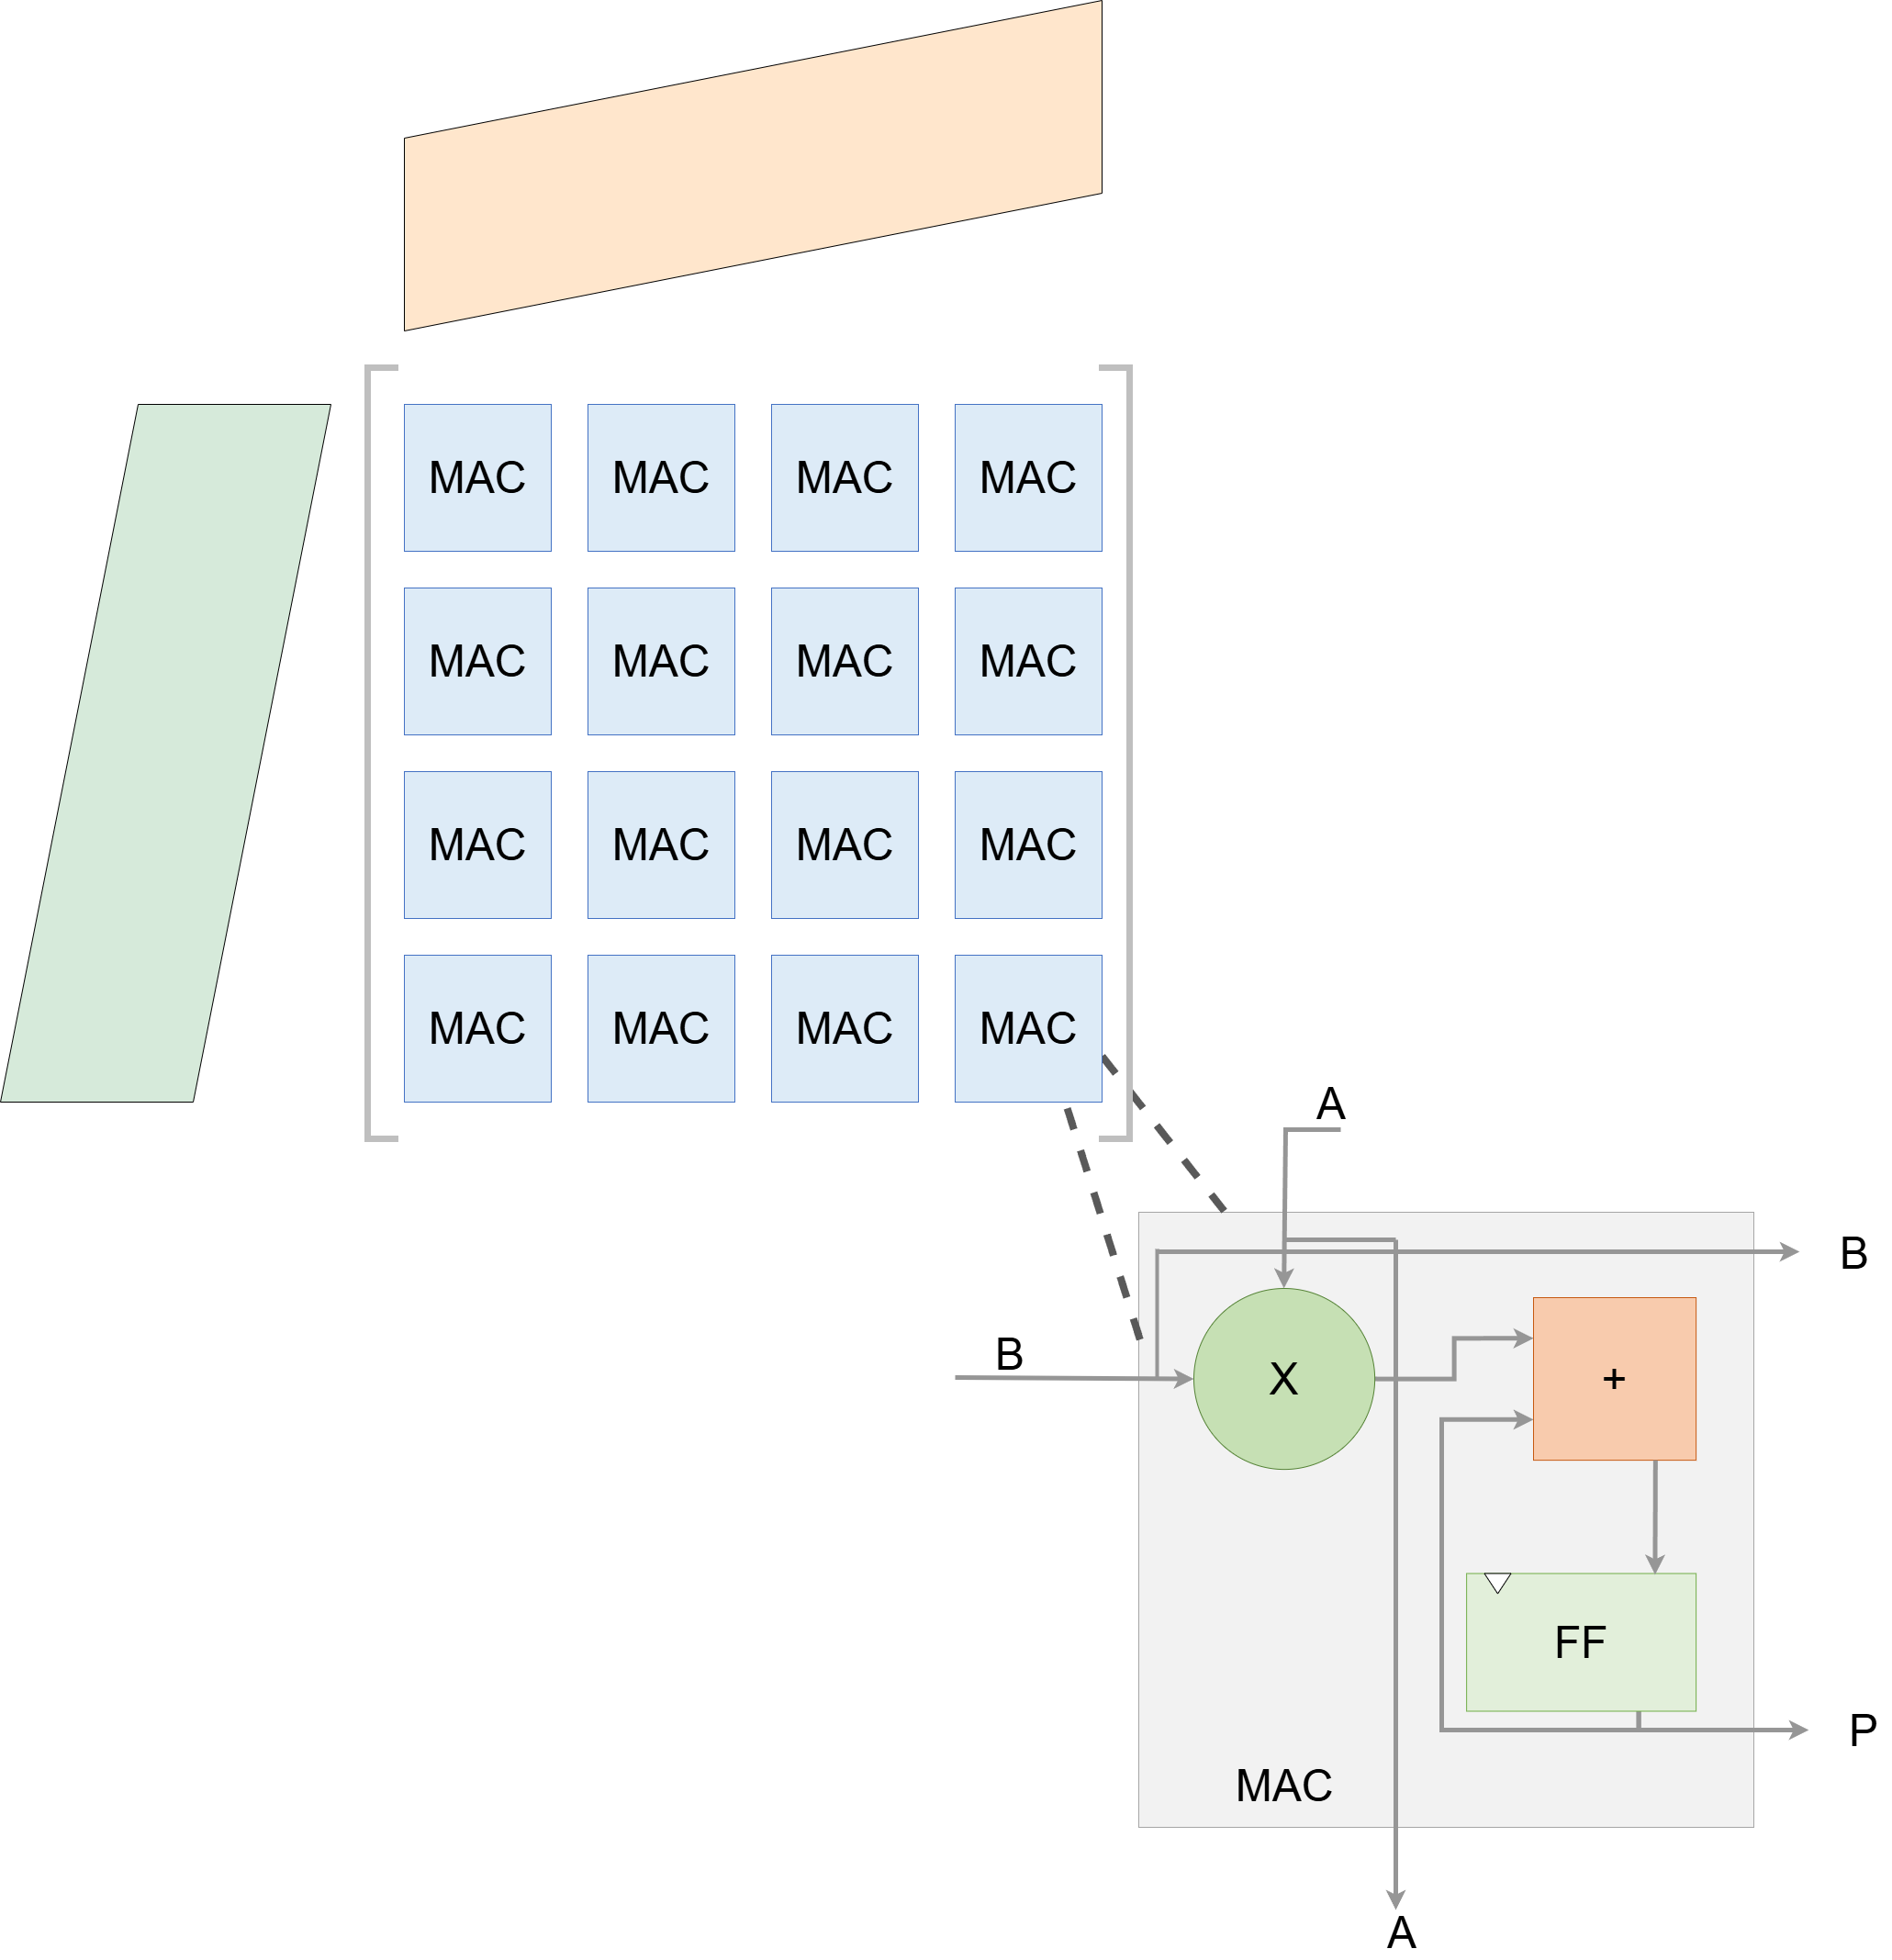
\includegraphics[scale = 0.15]{Figures/systolic_array_v2.png}}
	\caption{Systolic Array Architecture}
	\label{fig:systolic-array}
\end{figure}



%% END OF THE SECTION - MATRIX MULTIPLICATION TECHNIQUES ON HARDWARE %%

%% START OF THE SECTION - SINGULAR VALUE DECOMPOSITION ON HARDWARE %%
\section{Singular Value Decomposition on Hardware}
Singular value decomposition (SVD) is a fundamental operation in numerous scientific and engineering domains; however, its computational complexity poses substantial challenges, particularly for large-scale matrices. Two prominent approaches for computing SVD are the Jacobi algorithm and the Golub-Kahan algorithm, each possessing distinct computational characteristics and implications for hardware acceleration. The Jacobi algorithm, in both its one-sided and two-sided variants, iteratively applies Givens rotations to nullify off-diagonal elements, progressively transforming the matrix into diagonal form\cite{svd_architecture-6}. Singular values emerge along the diagonal, while the corresponding singular vectors are accumulated via successive orthogonal transformations. A notable advantage of the Jacobi method is its intrinsic parallelism, allowing Givens rotations to be applied independently to different matrix elements, thereby facilitating efficient concurrent execution. This parallel structure renders the Jacobi algorithm particularly well-suited for hardware acceleration on FPGAs, GPUs, and custom ASICs, where parallel computing resources can be fully utilized to expedite convergence.

Conversely, the Golub-Kahan algorithm employs a fundamentally different strategy by first reducing the matrix to a bidiagonal form via Householder reflections, followed by iterative QR decomposition to compute singular values\cite{svd-hardware-1}. An example of the Golub-Kahan algorithm was implemented in \cite{svd-hardware-2}, where the SVD was accelerated in Orthogonal Frequency Division Multiplexing (OFDM) for Multiple Signal Classification. This two-stage process introduces sequential dependencies that constrain parallelization. While the bidiagonalization phase ensures numerical stability, it involves substantial memory movement and matrix-vector multiplications, which present a bottleneck in hardware implementations. Furthermore, the QR iteration phase operates on the entire bidiagonal structure rather than individual matrix elements, leading to increased computational complexity and limited parallel execution capabilities. These inherent constraints make the Golub-Kahan algorithm less attractive for hardware implementations where efficiency and parallelism are paramount.

A key advantage of the Jacobi algorithm over Golub-Kahan is its superior numerical stability, particularly in handling ill-conditioned matrices. In numerical computations, ill-conditioned matrices exhibit small singular values that are highly sensitive to perturbations. The Jacobi method, leveraging iterative orthogonal transformations, ensures high precision in singular value computation while minimizing the accumulation of rounding errors. Each Givens rotation operates on a localized subset of matrix elements, thereby maintaining numerical accuracy throughout the transformation process. Conversely, the Golub-Kahan algorithm, particularly during its QR iteration phase, is susceptible to numerical instability due to repeated matrix factorizations, which amplify rounding errors over successive iterations. Consequently, the Jacobi approach is preferable for applications requiring high-precision singular value computations, including signal processing, control systems, and machine learning\cite{svd-hardware-3}.

From a hardware implementation perspective, the Jacobi algorithm aligns well with systolic array architectures, which are commonly employed for accelerating linear algebra computations. The ability to apply Givens rotations in parallel across multiple off-diagonal elements facilitates the design of highly efficient systolic arrays, where each processing unit performs localized transformations while maintaining communication with neighboring units. This distributed computation model significantly enhances throughput and reduces latency relative to sequential methodologies\cite{svd-hardware-4}. In contrast, the Golub-Kahan algorithm’s reliance on sequential bidiagonalization and QR factorization impedes efficient mapping onto systolic architectures, making it less desirable for FPGA and ASIC implementations.

Furthermore, the Jacobi algorithm’s reliance on element-wise transformations, rather than explicit matrix multiplications, leads to lower memory bandwidth requirements—a critical advantage in hardware accelerator design. Memory bandwidth often constitutes a limiting factor in high-performance computing applications, and minimizing data movement is essential for achieving energy efficiency and high-speed execution. The Golub-Kahan method, in contrast, involves multiple matrix-vector multiplications during the bidiagonalization process, exacerbating memory access demands and reducing suitability for low-power, high-efficiency hardware architectures.

Given these advantages, the Jacobi algorithm emerges as the preferred choice for hardware-accelerated SVD computation, particularly in FPGA- and ASIC-based systems. Its high parallelizability, superior numerical stability, efficient memory utilization, and compatibility with systolic architectures render it an optimal candidate for large-scale matrix computations in domains such as machine learning, image processing, and scientific computing. While the Golub-Kahan algorithm remains a robust option for general-purpose CPU-based implementations, its sequential constraints and elevated memory demands render it suboptimal for dedicated hardware acceleration scenarios.

\subsection{Jacobi Eigenvalue Decomposition}
The goal of PCA is to compute the eigenvalues and eigenvectors of the covariance matrix of a dataset. The Jacobi algorithm accomplishes this by iteratively applying orthogonal transformations to diagonalize the matrix.

The Jacobian Eigenvalue algorithm is presented below-
\begin{enumerate}
	\item \textbf{Input:} A symmetric covariance matrix \( C \) of dimension \( N \) x \( N \)
	\item Initialise the Eigenvector matrix \( V \) = \( I \). This matrix would accumulate the rotations
	\item Identify indices \( p \) and \( q \) such that  \( |c_{pq}| \) is the largest off diagonal element. The element would be reduced to zero in subsequent rotations
	\item Compute the rotation angle \( \theta \), that would zero out \( c_{pq} \). This is given by the equation \( 2\theta = \frac{2c_{pq}}{c_{pp} - c_{qq}} \)
	\item Calculate the value of \( cos(\theta) \) and \( sin(\theta) \)
	\item Construct an identity matrix \( R_{pq} \), and modify it such that \( R_{pp} = cos(\theta) \), \( R_{pq} = sin(\theta) \), \( R_{qp} = -sin(\theta) \), \( R_{qq} = cos(\theta) \)
	\item Apply the rotation as described by the equation \( C^{'} = R^{T}_{pq}CR_{pq} \)
	\item Update the Eigenvector Matrix \( V = VR \)
	\item The algorithm converges when all the off diagonal elements of \( C \) are below a specified tolerance \( \epsilon \)
	\item Columns of \( V \) are Eigenvectors
	\item \textbf{Output:} Return the Eigenvalue Decomposition of \( C \).
\end{enumerate}

Hence The Jacobian algorithm is the prefferred choice for hardware accelerator SVD computation. Particulary in FPGA and ASIC board systems\cite{svd-hardware-5}. Its highly parallelizable in nature superior numerical stability, efficient memory usage, and compatibility with systolic array architectures make it an ideal candidate for large - scale matrix computations in applications such as machine learning, image processing and scientific computing. 

%% END OF THE SECTION - SINGULAR VALUE DECOMPOSITION ON HARDWARE %%

%% START OF THE SECTION - INTRODUCTION TO CORDICs %%
\section{Introduction to CORDICs}
The Coordinate Rotation Digital Computer (CORDIC) algorithm is a highly efficient iterative method used for computing a variety of mathematical functions, including trigonometric, hyperbolic, logarithmic, and exponential functions. Developed by Jack Volder in 1959\cite{cordic-3} and later extended by Walther, CORDIC is particularly well-suited for hardware implementations such as Field Programmable Gate Arrays (FPGAs) and Application-Specific Integrated Circuits (ASICs) due to its ability to perform computations using only shift-and-add operations, avoiding the need for costly multipliers. This makes CORDIC an essential building block in digital signal processing (DSP), computer graphics, and scientific computing applications where real-time performance and efficient hardware utilization are critical. The algorithm operates by performing a sequence of iterative micro-rotations to approximate the desired function, making it particularly useful in FPGA-based architectures where hardware efficiency and low power consumption are crucial\cite{cordic-1}.

The CORDIC algorithm is based on the principle of vector rotation in a Cartesian coordinate system. Given an initial vector \( (x_{0}, y_{0}) \), the goal is to rotate it by an angle \( \theta \) to obtain a new vector \( (x^{'}, y^{'}) \) without using multiplication operations. This is accomplished by performing a series of micro-rotations of fixed angles that converge to the desired rotation. The core mathematical equations governing CORDIC in rotation mode are:
% CORDIC Equation-1
\begin{equation}
	\label{eq:equation_3}
	x_{i+1} = x_{i} - y_{i}d_{i}2^{-1}
\end{equation}

% CORDIC Equation-2
\begin{equation}
	\label{eq:equation_3}
	y_{i+1} = y_{i} + x_{i}d_{i}2^{-1}
\end{equation}

% CORDIC Equation-3
\begin{equation}
	\label{eq:equation_3}
	z_{i+1} = z_{i} - d_{i}tan^{-1}(2^{-1})
\end{equation}

where \( x_{i} \) and \( y_{i} \) are the coordinates of the vector in iteration \( i \), \( z_{i} \) is the angle that is progressively reduced to zero, \( d_{i} \) is the direction, determined as \( d_{i} = sign(z_{i}) \) ensuring that the angle is reduced in magnitude at each step. Here, \( 2^{-i} \) represents the micro-rotation scaling factor and \( tan^{-1}(2^{-i}) \) represents the precomputed constant for each iteration.

The iterative nature of the CORDIC algorithm means that each step rotates the vector by a smaller angle, refining the approximation with each iteration. Since multiplication by \( 2^{-i} \) is equivalent to a right bitwise shift, the entire computation involves only additions and shifts, making it extremely hardware-friendly.

CORDIC is particularly well-suited for FPGA-based hardware acceleration due to its shift-and-add architecture. Many FPGA vendors, including Xilinx and Intel, provide optimized CORDIC IP cores that can be easily integrated into hardware designs\cite{cordic-2}. The implementation consists of a series of iterative processing units, each responsible for executing one iteration of the algorithm. These units are pipelined to improve throughput, allowing multiple computations to be performed simultaneously.

% Cordic rotation angle Image
\begin{figure}[H]
	\centerline{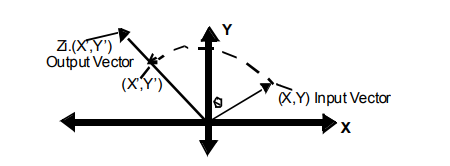
\includegraphics[scale = 0.80]{Figures/AMD_1.png}}
	\caption{CORDIC Rotation}
	\label{cordic rotation}
\end{figure}


%% END OF THE SECTION - INTRODUCTION TO CORDICs %%

%% START OF THE SECTION - CACHE ARCHITECTURE AND MODELING %%
\section{Cache Architecture and Modeling}
The performance of compute-bound and memory-bound applications, particularly in machine learning and signal processing accelerators, is significantly impacted by memory hierarchy efficiency. Cache design, including mapping strategies, write policies, and cache modeling techniques, plays a central role in improving data locality, reducing access latency, and optimizing energy use. This section explores foundational cache architectures, behavioral policies for write misses, real-world benchmarks used for cache modeling, and the use of CACTI for memory subsystem analysis.

\subsection{Direct Mapped Caches}
A direct-mapped cache, as shown in Fig.\ref{fig:direct-mapped-cache-arch}, represents the simplest form of address mapping in cache memory, where each block in main memory is mapped to exactly one location (or set) in the cache. Address decomposition in this cache type typically includes three fields: offset, index, and tag. The index field selects a unique cache line, and the tag is used to validate that the correct data is stored in that line. While this makes the design low-overhead and fast in lookup, it introduces potential issues with conflict misses, particularly if multiple memory addresses map to the same index\cite{cache-1}.

\begin{figure}
	\centerline{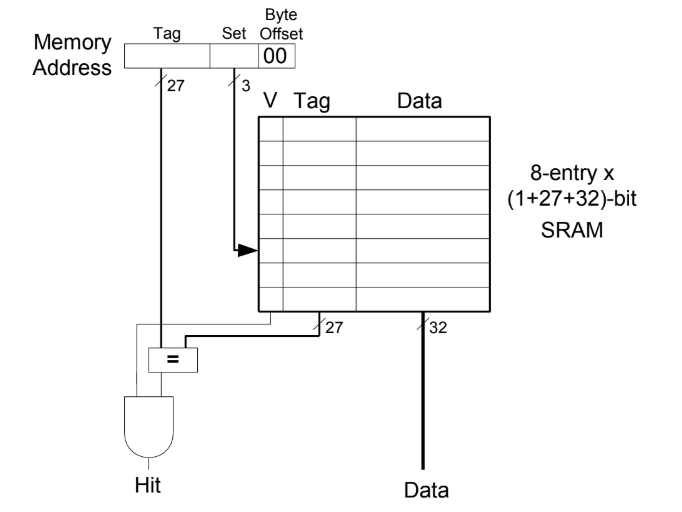
\includegraphics[scale = 0.6]{Figures/direct_mapped_cache_architecture.png}}
	\caption{Architecture of a Direct-Mapped Cache}
	\label{fig:direct-mapped-cache-arch}
\end{figure}

Despite their simplicity, direct-mapped caches can perform competitively when the access pattern exhibits high spatial locality and low contention. In FPGA-based accelerators, where deterministic timing is often more important than average-case throughput, direct-mapped caches offer predictable timing behavior and are easier to implement with minimal logic resources. However, for applications with large and irregular access footprints, such as matrix multiplication or sparse data reads, they may become a performance bottleneck due to frequent evictions.

\subsection{Cache Write Miss Policies}
\subsubsection{Write-Allocate Write-Miss Policy}
The write-allocate (also called fetch-on-write) policy dictates that when a write miss occurs, the block is first loaded from memory into the cache, and then the write is performed on the newly cached block. This policy assumes that the data being written is likely to be accessed again soon, benefiting from temporal locality. Write-allocate is usually combined with write-back, which reduces the number of memory write operations by deferring them until cache eviction.

In the context of FPGA accelerators for ML inference or training tasks, this policy is particularly useful when intermediate results — such as partial matrix products or activation values — are updated iteratively and accessed multiple times across computation cycles. By ensuring such values remain in the cache after being written, write-allocate reduces memory access latency and minimizes redundant memory transactions\cite{cache-3}.

Nonetheless, write-allocate incurs additional latency on write misses, as the cache line must first be fetched before the store can proceed. For latency-sensitive paths, this may create pipeline stalls or increase critical path pressure.

\subsubsection{Write-Around Write-Miss Policy}
In contrast, the write-around policy does not bring the missed data block into the cache. Instead, it bypasses the cache and writes directly to main memory. This is advantageous in workloads where written data is not expected to be reused, such as logging, streaming, or forward-only computations. By avoiding unnecessary cache fills, write-around reduces cache pollution, freeing up lines for data with higher reuse potential.

Write-around is often used alongside write-through caching, which ensures all writes update main memory immediately, preserving coherence across memory hierarchies. In FPGA accelerators like Manojavam, this policy is ideal for RHS matrix tiles in matrix multiplication, which are streamed in, used exactly once, and then discarded\cite{cache-3}.

However, write-around increases main memory bandwidth usage and may reduce energy efficiency if employed indiscriminately. It is best suited for write-once, read-never access patterns that dominate many preprocessing or forward-propagation stages in ML pipelines\cite{cache-4}.

\subsection{Cache Modeling Benchmarks}
Evaluating the effectiveness of cache policies requires realistic memory access patterns. Two well-established benchmark suites — LINPACK SAXPY and Livermore Loops — are used in this study to simulate cache behavior under practical conditions.

\subsubsection{LINPACK SAXPY Benchmark}
The SAXPY kernel (Single-Precision A·X Plus Y) is a Level-1 BLAS operation, represented by the equation:
\begin{equation}
	Y[i] = A.X[i] + B.Y[i]
\end{equation}

This pattern combines sequential reads from two input vectors with a write-back into one, making it ideal for testing read-write mixing, line reuse, and miss handling. In cache simulations, SAXPY reveals how well a system supports regular, linear memory access patterns with temporal locality\cite{cache-5}.

\subsubsection{Livermore Benchmark}
The Livermore Fortran Kernels (LFK) consist of 24 small programs, each designed to model a different class of scientific computation. These include operations like matrix multiplication, vector updates, numerical integration, and particle simulation. The Livermore benchmark of interest in this study, is given in the following equation-
\begin{equation}
	Z[i] = A.X[i] + B.Y[i]
\end{equation}

This equation involves multiple simultaneous memory reads, multiplication, and a final update, mimicking compute stages where multiple operands must be fetched concurrently. The reuse distance, line alignment, and miss rate behavior of this kernel provide deep insights into how the cache hierarchy responds to nested loops and indirect accesses.

Livermore Loops are especially useful for stress-testing multi-port caches, bank conflicts, and stride-sensitive performance — traits that become critical in loop-unrolled ML workloads\cite{cache-6}.

\subsection{CACTI Cache Modeler}
CACTI (Cache Access and Cycle Time Infrastructure) is a comprehensive tool for modeling cache and memory subsystems with respect to access latency, power consumption, and physical area. Originally developed by Hewlett-Packard Labs and later expanded by researchers at the University of Utah, CACTI has become a widely used framework for evaluating SRAM-based cache designs in both research and industrial contexts. It allows designers to explore how microarchitectural decisions — such as cache size, associativity, block size, number of ports, and banking — affect delay, energy, and silicon footprint\cite{cache-7}\cite{cache-8}.

At a high level, CACTI combines delay models for SRAM cells and peripheral logic with power and area estimators derived from accurate transistor-level characterizations. It simulates the read and write paths through the memory array, including precharge, sense amplification, wordline and bitline transitions, tag comparison, and output drivers. These computations are further refined by incorporating RC interconnect delay models for local and global wiring, providing timing estimates that closely reflect physical implementation constraints.

The tool accepts a range of parameters including total cache size, line size, associativity, number of banks and ports, and the target technology node. From this, it produces detailed reports on access latency, cycle time, dynamic and leakage power, and layout area. CACTI also supports different access modes — including sequential, fast, and normal — each modeling different levels of precharge and comparator overlap.

By enabling rapid design-space exploration across technology generations and architectural configurations, CACTI facilitates early-stage memory subsystem planning. It is particularly useful when evaluating trade-offs between latency, energy efficiency, and area — all of which are critical constraints in hardware accelerators, embedded processors, and SoC memory hierarchies. Its extensibility and compatibility with open-source flows make it an ideal modeling tool for cache-centric hardware research.

%% END OF THE SECTION - CACHE ARCHITECTURE AND MODELING %%

%% START OF THE SECTION - FPGA DESIGN FLOW %%
\section{FPGA Design Flow}
The FPGA design flow is a comprehensive process that transforms a high-level hardware description into a physical configuration bitstream, allowing the FPGA device to behave as the intended digital circuit. This multi-stage flow, as shown in Fig.\ref{fig:fpga-design-flow} is essential to ensure the design is functionally correct, meets timing requirements, and optimally utilizes hardware resources. Each stage builds upon the previous one, gradually refining the design until it is ready for deployment.

\begin{figure}[H]
	\centerline{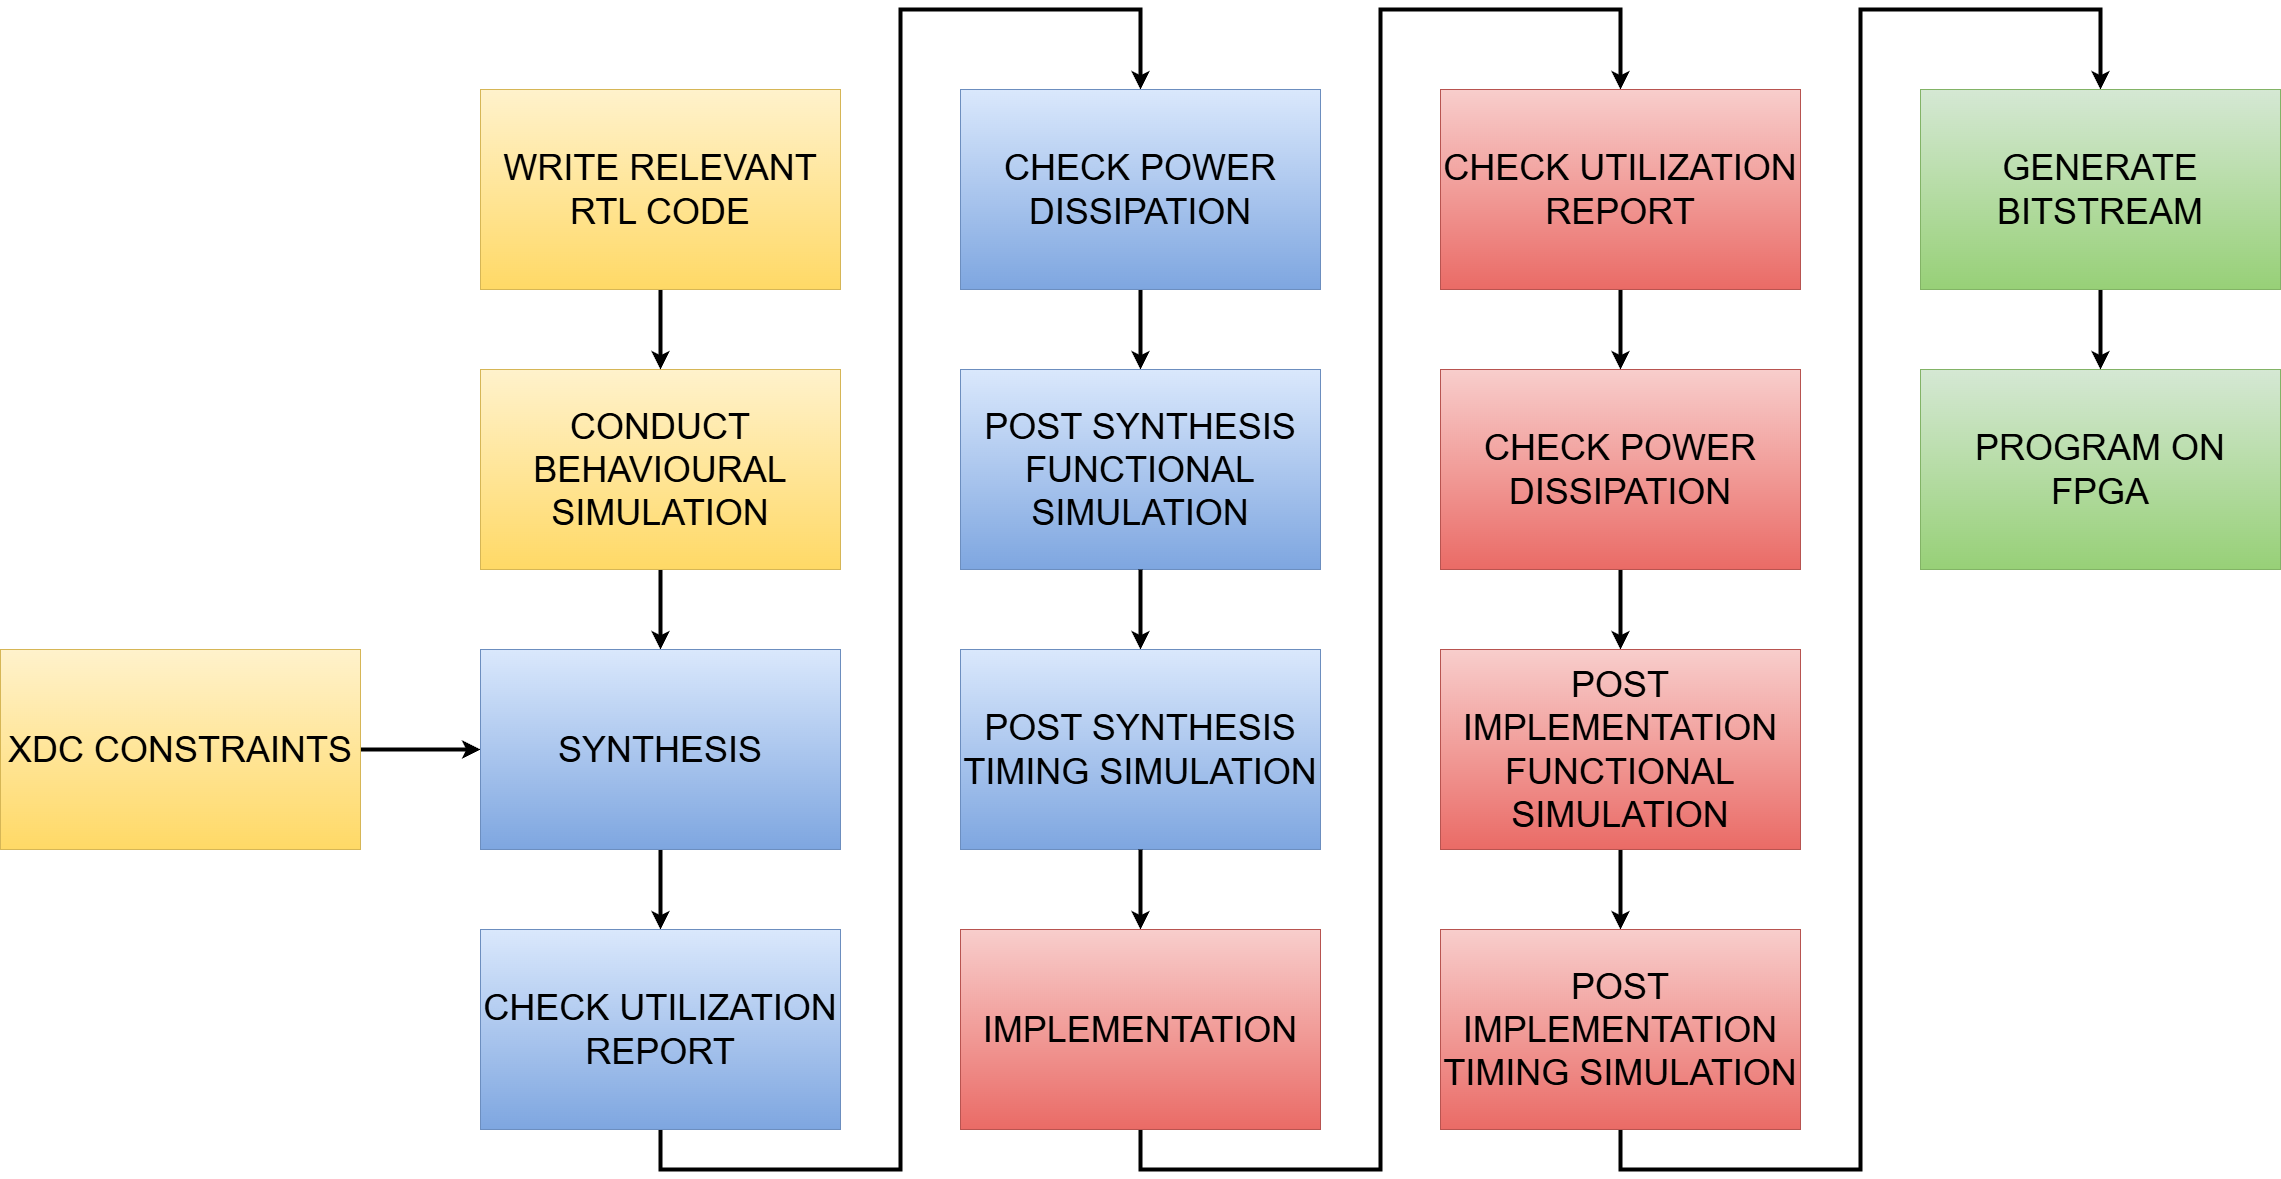
\includegraphics[scale = 0.2]{Figures/FPGA_design_flow_v2.png}}
	\caption{FPGA Design Flow}
	\label{fig:fpga-design-flow}
\end{figure}

\subsection{RTL Entry}
Register Transfer Level (RTL) entry represents the first and foundational step in the FPGA design process. Here, the digital system's behavior and structure are described using a hardware description language (HDL), most commonly Verilog or VHDL. The RTL abstraction focuses on the flow of data between registers and the operations performed on that data synchronized by clock signals.

Writing synthesizable RTL code requires deep understanding of digital logic design and coding guidelines to ensure that the code can be successfully transformed into hardware. Designers must focus on writing clean, modular, and reusable code with clear synchronous logic constructs, avoiding non-synthesizable constructs like delays or certain loops that can't be mapped to hardware. The RTL code typically includes the definition of combinational logic, synchronous state machines, arithmetic units, multiplexers, and register files.

This stage sets the design intent clearly and forms the basis for all subsequent synthesis and implementation steps. Good RTL design not only ensures functional correctness but also heavily influences the efficiency, speed, and area utilization of the final FPGA implementation.

\subsection{Behavioural Simulation}
Behavioral simulation is the process of verifying the RTL code at a functional level before any hardware synthesis or physical mapping. It is the first verification checkpoint, focused on confirming that the design logic behaves as expected under a wide range of input conditions without considering any timing delays.

In this phase, simulation testbenches are written to provide input stimuli and monitor outputs. Testbenches model realistic operating scenarios, edge cases, and corner conditions to verify the correctness of control paths, data paths, and overall system behavior. Common simulation environments include ModelSim, QuestaSim, and Vivado Simulator.

Behavioral simulation supports iterative debugging, allowing designers to detect and fix logic bugs early, thereby reducing the risk of expensive errors downstream. It also facilitates the validation of complex algorithms and state machine transitions before the design is locked for synthesis. This step is crucial to build confidence that the design will function correctly once synthesized and implemented.

\subsection{Synthesis}
Synthesis is a pivotal step where the RTL code is automatically translated into a gate-level representation compatible with the FPGA's architecture. This process converts abstract behavioral descriptions into an optimized network of logic gates, lookup tables (LUTs), flip-flops, multiplexers, and embedded blocks like DSP slices and block RAMs.

The synthesis tool, such as Xilinx Vivado or Synplify Pro, analyzes the RTL for logic equivalence, timing, and resource constraints, then performs optimizations including logic minimization, retiming, and resource sharing. The synthesis output is a Technology Mapped Netlist (TMNL) — a detailed description of the design using the primitives available in the target FPGA device.

The synthesis process also provides crucial reports indicating estimated resource utilization (LUTs, FFs, DSPs, BRAMs), maximum achievable clock frequency, and warnings or errors. Designers can tweak the RTL code or synthesis constraints to improve performance or reduce resource usage. A well-optimized synthesis directly influences the quality of results (QoR) of the overall design.

\subsection{Post Synthesis Simulation}
Once synthesis completes, post-synthesis simulation serves as the next verification stage to ensure that the synthesized netlist preserves the intended functionality of the RTL. Unlike behavioral simulation, this step uses the gate-level netlist and incorporates basic gate delays and timing models that reflect the synthesis tool’s understanding of the hardware implementation.

The simulation includes detailed signal propagation through logic gates and flip-flops, enabling detection of functional discrepancies introduced during synthesis optimization such as logic restructuring or resource sharing. Post-synthesis simulation helps verify that the design’s logical correctness remains intact and is crucial before committing to the implementation stage.

Additionally, this simulation helps designers spot issues related to glitches, race conditions, or unexpected logic behavior caused by gate-level transformations. It sets the foundation for accurate timing analysis and confirms that the design is ready for the more detailed physical implementation flow.

\subsection{Implementation}
Implementation is the stage where the synthesized netlist is physically mapped, placed, and routed onto the FPGA fabric. It consists of several intricate sub-steps that translate the logical design into a physical layout optimized for speed and resource utilization.
\begin{enumerate}
	\item \textbf{Translation:} Converts the synthesized netlist and constraints into a format suitable for implementation tools.
	\item \textbf{Mapping:} Assigns the synthesized logic elements like LUTs, flip-flops, DSP blocks, and BRAMs to the physical resources available on the FPGA device.
	\item \textbf{Placement:} Strategically determines the exact physical locations on the FPGA for each logic element, balancing the trade-offs between performance, congestion, and resource distribution. Placement algorithms aim to minimize critical path delays and interconnect complexity.
	\item \textbf{Routing:} Establishes physical connections between placed elements through the FPGA’s programmable routing fabric. Routing ensures that signals meet timing requirements and avoids routing congestion and cross-talk.
\end{enumerate}

This stage involves iterative optimization driven by timing constraints and resource availability specified in the constraints file. Modern FPGA tools use advanced heuristics and machine learning-based algorithms to find near-optimal placement and routing solutions.

Implementation generates detailed timing reports and resource utilization metrics. Achieving timing closure — meeting all timing constraints such as setup and hold times — is one of the most challenging aspects of the implementation phase.

\subsection{Post Implementation Simulation}
Post-implementation or timing simulation models the design’s behavior with full consideration of the detailed delays introduced by the actual physical placement and routing. This simulation uses the timing back-annotated netlist (SDF file) containing precise delay values for all interconnects and logic elements, reflecting the true operating conditions on the FPGA.

This stage verifies that the design meets timing constraints under worst-case delay scenarios and functions correctly with actual path delays, clock skews, jitter, and other physical effects. It helps identify timing violations, race conditions, and glitches that could lead to functional failures in silicon.

Post-implementation simulation is often the final functional verification step before generating the FPGA bitstream. Passing this simulation provides confidence that the design will operate reliably at the targeted clock frequency once programmed on the device.

\subsection{Xilinx Design Constraints}
The Xilinx Design Constraints (XDC) file is a vital input to synthesis and implementation tools, specifying the physical and timing requirements of the design. The XDC file uses the industry-standard Synopsys Design Constraints (SDC) syntax and allows precise control over various aspects of the FPGA implementation\cite{fpga-flow-1}.

Key components of an XDC file include:
\begin{enumerate}
	\item \textbf{Pin Assignments:} Mapping logical signals to specific FPGA I/O pins, ensuring correct electrical connections to external hardware interfaces such as sensors, memory modules, or communication lines.
	\item \textbf{Clock Definitions:} Specification of clock signals including frequency, duty cycle, waveform timing, and clock groups to guide timing analysis and optimization.
	\item \textbf{Timing Constraints:} Setup and hold time requirements, false path and multi-cycle path declarations, and exceptions that allow the tools to focus on critical timing paths.
	\item \textbf{Placement Constraints:} User directives for floorplanning, such as locking down specific logic blocks or I/O to fixed locations to optimize performance or meet design partitioning goals.
	\item \textbf{Physical Constraints:} Constraints related to voltage standards, slew rates, drive strengths, and other electrical characteristics. 
\end{enumerate}

Accurate and comprehensive constraints in the XDC file are essential for ensuring the design meets functional, timing, and interface specifications in the final FPGA implementation.

\subsection{Bitstream Generation}
Bitstream generation is the culminating step in the FPGA design flow, where the fully implemented design is converted into a binary configuration file that programs the FPGA device. This bitstream encodes all information regarding logic configurations, routing paths, clock setups, and I/O assignments, essentially ‘telling’ the FPGA how to physically realize the design.

The bitstream is generated by the FPGA vendor tools once timing closure is confirmed and the implementation results are satisfactory. The tool packages the design into a format compatible with the target FPGA device’s configuration memory, considering encryption, compression, and device-specific requirements.

After bitstream generation, the file is loaded onto the FPGA via programming interfaces such as JTAG, SPI, or Platform Cable USB. Once programmed, the FPGA starts operating as the designed digital system.

This final step is critical as any errors or timing violations detected after bitstream generation require returning to earlier design stages for correction. Successful bitstream generation signifies the completion of the FPGA design process and readiness for hardware testing and deployment.

%% END OF THE SECTION - FPGA DESIGN FLOW %%

%% START OF THE SECTION - ASIC DESIGN FLOW ON OPENLANE AND OPENRAM %%
\section{ASIC Design Flow on Openlane and OpenRAM}
ASIC design transforms RTL descriptions into manufacturable silicon layouts through a sequence of design stages. OpenLane, developed by the OpenROAD project\cite{asic-3}, is an open-source, fully automated ASIC backend flow that integrates various open-source EDA tools to streamline this process\cite{asic-1}. OpenRAM complements OpenLane by providing an open-source SRAM compiler, enabling automated generation of memory blocks essential for many ASIC designs\cite{asic-2}.

\subsection{Openlane Architecture and Flow}
OpenLane orchestrates the ASIC backend implementation starting from synthesized RTL and design constraints, producing a final verified layout. It integrates tools such as Yosys for synthesis, OpenDP for placement, TritonRoute for routing, and OpenSTA for timing analysis, all managed via Python scripts and containerized environments for reproducibility. The Openlane ASIC flow is depicted in Fig.\ref{fig:openlane-flow}.

\begin{figure}[H]
	\centerline{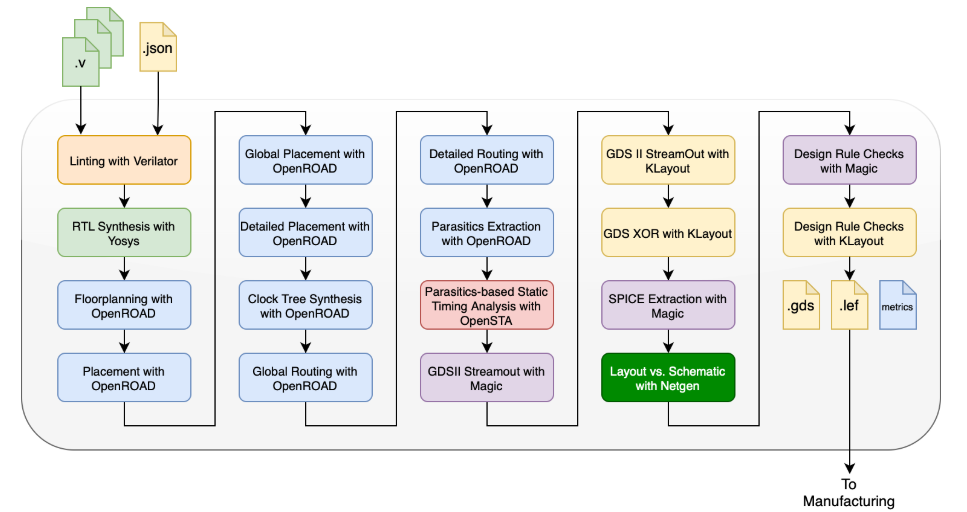
\includegraphics[scale = 0.75]{Figures/openlane_flow.png}}
	\caption{ASIC Openlane Flow\cite{asic-1}}
	\label{fig:openlane-flow}
\end{figure}

The key stages include-
\begin{enumerate}
	\item \textbf{Synthesis:} Converts RTL into a gate-level netlist optimized for the target technology.
	\item \textbf{Floorplanning:} Defines core area, I/O placement, and power grid setup.
	\item \textbf{Placement and Clock Tree Synthesis:} Assigns physical locations to cells and synthesizes the clock distribution network.
	\item \textbf{Routing:} Connects cells with metal layers while ensuring design rule compliance.
	\item \textbf{Verification:} Performs DRC, LVS, and static timing analysis.
	\item \textbf{GDSII Generation:} Creates the final layout file for fabrication.
\end{enumerate}

OpenLane uses YAML-based configuration files to customize design parameters such as technology libraries, floorplan dimensions, and clock frequencies, providing flexibility across different ASIC projects.

\subsection{OpenRAM Integration}
OpenRAM is a parameterizable, open-source SRAM compiler that automatically generates synthesizable RTL, physical layout, and timing models tailored to specified memory configurations like size, port count, and banking.

OpenRAM SRAM blocks integrate smoothly into the OpenLane flow by:
\begin{enumerate}
	\item Being instantiated directly in RTL or added post-synthesis as black-box macros.
	\item Undergoing placement and routing alongside standard cells during implementation.
	\item Providing accurate timing and power characterization models to assist timing closure and power estimation.
\end{enumerate}

This integration eliminates the need for manual SRAM design, accelerating ASIC development and improving design reliability.

%% END OF THE SECTION - ASIC DESIGN FLOW ON OPENLANE %%

\begin{comment}

\section{Use of Acronyms and Glossaries}
Acronyms are nothing but the short form of regular repeated word. Say for example, you have a repeat word "Integrated Circuits" and you want to use a short form for it as "IC". For which you have to first define the word and use it wherever you wanted to refer it.

First, let's look at the definition, which has to be entered in \texttt{Glossaries.tex} under \texttt{CoverPages} directory.
\begin{verbatim}
%\newacronym{<Ref>}{<Short-Form>}{<Expanded word>}
\newacronym{ic}{IC}{Integrated Circuits}
\end{verbatim}
In order to use the defined acronym, use the commands \verb|\gls{<Ref>}| as shown below

As an example, call the definition with \verb|\gls{ic}| and the outcome of it is reflected as, \gls{ic}.

Note: For the First time, the expanded form appears along with the Short-form definition inside parenthesis. But when the \verb|\gls{}| is repeated, only Short-form appears inside the parenthesis.

Now, let's look at the definition of symbols. Follow the syntax to define the symbol first, inside \texttt{Glossaries.tex} under \texttt{CoverPages} directory.
\begin{verbatim}
%\newglossaryentry{<Ref>}{name=<Symbol>, description={<description about the symbol>}, type=<List type>}
\newglossaryentry{rc}{name=$\tau$, description={Time constant}, type=symbolList}
\end{verbatim}

As an example, the rate of change is defined with \verb|\gls{rc}| and the outcome of it is reflected as, the rate of change is defined with \gls{rc}.

\vspace{0.75cm}

 \textbf{The chapters should not end with figures, instead bring the paragraph explaining about the figure at the end followed by a summary paragraph.}


After elaborating the various sections of the chapter (From Chapter 2 onwards), a summary paragraph should be written discussing the highlights of that particular chapter. This summary paragraph should not be numbered separately. This paragraph should connect the present chapter to the next chapter.
\end{comment}

This chapter outlined the essential theoretical and technical foundations supporting the two key aspects of the project: FPGA architectural exploration and the RTL-to-ASIC design of the Manojavam PCA accelerator. The FPGA section began by examining the internal structure of FPGAs, focusing on Configurable Logic Blocks (CLBs), lookup tables (LUTs), and routing elements such as switch boxes. It introduced the baseline Intel Stratix-10 architecture along with custom 4-bit Single and Double Carry Chain architectures optimized for low-precision arithmetic and parallel carry propagation. The importance of area, delay, and logic utilization as evaluation metrics was discussed in the context of machine learning hardware acceleration. The VTR toolchain was detailed, emphasizing the roles of Yosys (for Verilog synthesis), ABC (for logic optimization and technology mapping), and VPR (for packing, placement, routing, and analysis), along with the use of architecture description XML files for architectural specification.

The second part of the chapter focused on the Manojavam PCA accelerator, starting with matrix multiplication strategies that use 4×4 operand tiling and controller-driven tile streaming. It introduced systolic arrays based on TPU-style architectures and explained both weight-stationary and output-stationary dataflows to maximize throughput and regularity. The mathematical basis of PCA was discussed through covariance matrix formulation and the Jacobi method, highlighting the role of Givens rotations in eigendecomposition. Memory hierarchy design was explored through a block-streamed structure with private L1 and shared L2 caches, incorporating write-around and write-validate policies. The RTL design process was explained using Verilog and Vivado, covering simulation, synthesis, implementation, and power-timing analysis. The ASIC design flow was covered through OpenLane, detailing floorplanning, placement, routing, and GDSII generation, along with OpenRAM-based SRAM integration. Supporting tools such as CACTI and a custom simulator were used for cache modeling and compute latency analysis. Altogether, these foundations established the architectural, algorithmic, and tool-driven context necessary for the development and evaluation of the project's hardware systems.
